%debugging
%\errorcontextlines=200
\documentclass[french, 12pt, twoside, openright, a4paper]{report}
%for left chapter titles add openright to report
\usepackage[utf8]{inputenc}
\usepackage{lmodern}
\usepackage[T1]{fontenc}
\usepackage[french]{babel}
\usepackage{amsmath}
\usepackage{amsfonts}
\usepackage{amssymb}
\usepackage[hidelinks]{hyperref}
\usepackage{graphicx} %remove demo for final version
\usepackage{siunitx}

\usepackage{floatrow}
\floatsetup[table]{capposition=top} % caption position above table

\usepackage[dvipsnames]{xcolor}
\usepackage{subcaption}
\usepackage{tabularx}

%tableau en francais
\addto\captionsfrench{\def\tablename{\textsc{Tableau}}}

%nomenclature
\usepackage[notintoc, french, noprefix]{nomencl}
\makenomenclature
%run makeindex -s nomencl.ist -o main.nls main.nlo
%Units
%----------------------------------------------
\newcommand{\nomunit}[1]{%
\renewcommand{\nomentryend}{\hspace*{\fill}#1}}
%----------------------------------------------
\setlength\nomlabelwidth{1.5cm}
\renewcommand{\nomname}{Nomenclature}

%circuits
\usepackage{tikz, circuitikz}
\usepackage{tkz-euclide}
\usetkzobj{all}
\usetikzlibrary{arrows.meta}

%pseudocode
\usepackage[ruled,longend]{algorithm2e}

%wrapping figures
\usepackage{wrapfig}

%TIMES NEW ROMAN FONT
\usepackage{mathptmx}
%\usepackage{charter}

% Python syntax highlighting
\usepackage{minted}
\usepackage{listings}
\usepackage{pythonhighlight}

%\setsansfont{Calibri}
%\setmonofont{Consolas}


\usepackage[a4paper, left=2cm, right=2cm, top=1.5cm, bottom=2cm]{geometry}

%check font size
\makeatletter
\newcommand\thefontsize{The current font size is: \f@size pt} 
\makeatother
%to set chapter and section title font sizes
\usepackage{sectsty}
\chapterfont{\fontsize{16}{18}\selectfont}
\sectionfont{\fontsize{14}{16}\selectfont}
\subsectionfont{\fontsize{12}{14}\selectfont}

%BLUE COLOR
\definecolor{blue}{HTML}{00578a}

\setcounter{tocdepth}{3}

\begin{document}

  \renewcommand{\theFancyVerbLine}{\sffamily\textcolor[rgb]{0.5,0.5,0.5}{\scriptsize\arabic{FancyVerbLine}}}

  \begin{titlepage}

\noindent
\begin{minipage}{0.15\textwidth}
      
\includegraphics[width=\linewidth]{resources/uae.jpg}
\end{minipage}
\hfill
\begin{minipage}{0.5\textwidth}
  \begin{center}
    \textbf{\large Université Abdelmalek Essaadi}\\[0.3cm] % Name of your university/college
    \textbf{\large Faculté des Sciences et Techniques Tanger}\\[0.5cm] % Major heading such as course name
    \textbf{\large 2019/2020}\\[1.5cm]
  \end{center}
    
\end{minipage}
\hfill
\begin{minipage}{0.2\textwidth}
  
\includegraphics[width=\linewidth]{resources/fstt.png}
\end{minipage}

\vspace*{1.5cm}

\centering

\textbf{\textcolor{blue}{Projet de Fin d’Études}}\\[0.3cm]
\textbf{\textcolor{blue}{Master Sciences et Techniques}}\\[0.5cm]
\colorbox{gray!50}{\strut\makebox[\dimexpr \linewidth-2\fboxsep][c]{\textit{\textbf{Option : Génie Énergétique}}}}\\[2cm]


\fbox{
  \begin{minipage}{\dimexpr\textwidth-2\fboxrule-2\fboxsep-6pt}
    \textbf{\textit{Titre:}}
    \begin{center}
      \textbf{\Large Estimation des paramètres des cellules photovoltaïques}\\[.2cm]\phantom{}
    \end{center}
  \end{minipage}
}
\vspace{1cm}
\begin{center}
\textbf{\textcolor{blue}{Présenté par :}}\\[0.5cm]
\textbf{Youssef Kharchouf}\\[0.5cm]
\textbf{\textcolor{blue}{Date de soutenance : Juin 2020}}
\end{center}
  
\textbf{Devant le Jury :\hfill\phantom{}}\\[.5cm]
\setlength\extrarowheight{5pt} %ROW HEIGHT
    \begin{tabular*}{\textwidth}{|c|@{\extracolsep{\fill}}c|c|}
    \hline
       \textbf{\textit{Nom et Prénom}} & \textbf{\textit{Établissement}} & \textbf{\textit{Qualité}} \\
       \hline
        & & \textbf{\textit{Président}} \\
        \hline
        & & \textbf{\textit{Examinateur}} \\
        \hline
        & & \textbf{\textit{Encadrant Externe}} \\
        \hline
        \textbf{Dr. Adil Chahboun} & \textbf{FST de Tanger} & \textbf{\textit{Encadrant de la FST}} \\
        \hline
    \end{tabular*}

\vfill
\textit{\textbf{\textcolor{blue}{PFE effectué au:}}}\\
(Laboratoire ou Société ou Organisme)
\vfill
LOGO du Laboratoire ou de la Société ou de l’organisme, ....

\end{titlepage}

  \shipout\null
  \section*{Résumé}
Les cellules solaires photovoltaïques sont généralement modélisées avec un circuit électrique comprenant un certain nombre de paramètres.

\section*{Abstract}
Solar PV cells are generally represented by a lumped-element model with a set number of components which are represented by their parameters. These parameters are not readily available in manufacturer data-sheets despite being crucial to the accuracy of the model. A possible approach is to estimate these parameters using the Current-Voltage characteristic of a cell using numerical or analytic techniques. Metaheuristics such as Differential Evolution take the approach of an optimization with the objective function to be minimized being the error with experimental Current-Voltage data. This work is a comparative analysis between different combinations of methods such as Differential Evolution and Particle Swarm Optimization applied to the single and double diode models for various solar cell technologies. PSO is used to initially cover the entire multidimensional search space in order to find a region with global minimum, which is subsequently given to the DE algorithm in order to locate the solution with the best fitness within this region. A small tool implementing these methods has been developed using the Python programming language.

\section*{Nomenclature}
\noindent\textbf{GHG} \hfill Green House Gas \hfill Gaz à effet de serre\\
\textbf{DE} \hfill Differential Evolution \hfill \phantom{}\\
\textbf{$E_g$} \hfill Bandgap\\
\textbf{EQE} \hfill External Quantum Efficiency\\

\newpage
\tableofcontents
\newpage

\chapter*{Introduction Générale}
\label{sec:intro}
\addcontentsline{toc}{section}{\nameref{sec:intro}}
%inexhaustible en principe
L’épuisement des énergies fossiles et leur nature non-durable a conduit à la croissance rapide des énergies renouvelables comme sources alternatives d'énergie. L’énergie solaire est l’une de ces sources renouvelables les plus répandues et a prouvé son utilité dans plusieurs domaines d'applications grâce à sa nature quasiment inexhaustible en principe. Les technologies photovoltaïques en particulier ont fait l'objet intense d'étude de la part de la communauté scientifique depuis la première cellule en silicone cristallin à 6\% de Chapin et al. \cite{Chapin1954} en 1954. Ceci a entraîné une croissance considérable de l'industrie photovoltaïques. En fait, la capacité de production en PV a dépassé les 150GW \cite{iea2020} en 2019 (figure \ref{fig:ieapv}), ce qui correspond une croissance d'environ 100GW depuis 2014. Les décennies de recherche depuis la cellule de Chapin et al. visent généralement l'amélioration des cellules solaires \textit{(i)} en explorant les différentes architectures possibles des cellules, \textit{(ii)} en développant des matériaux qui permettent d'augmenter l'efficacité de conversion de l'énergie solaire incidente ou \textit{(iii)} en réduisant le coût du processus de production. La première génération des technologies PV se basait sur des wafer de Silicone comme matériau actif de conversion. La deuxième génération remplace le silicone avec des semi-conducteurs à couches minces, qui, parmi d'autres avantages, réduit considérablement les besoins en matières premières (silicone). Les troisièmes et futures générations comprennent les cellules organiques, Perovskite et les Quantum Dots et présentent des pistes d'investigations pour réduire davantage les coûts de production et augmenter l'efficacité de conversion.\\
Le principe de fonctionnement des cellules photovoltaïques a été discuté en profondeur dans la littérature \cite{Fraas2010,  Sze2006, Wenham2013}.
Les photons à énergie supérieure au bandgap du matériau semi-conducteur sont absorbé en transférant leur énergie aux électrons dans la bande de valence, ce qui leur permet de passer vers la bande de conduction en laissant un "trou" derrière. Le rôle du champ électrique présent dans la zone de déplétion des jonctions P-N est de séparer ces paires électron-trou et leur permettre de circuler à travers une charge extérieure. Toutefois, il y aurait toujours un plafond sur ce mécanisme de conversion "lumière $\rightarrow$ électricité" pour les cellules mono-jonction selon la limite Schockley-Queisser (SQ) \cite{Shockley1961}. Le modèle SQ postule que tous les photons à énergie supérieure au gap $E_g$ sont absorbés et que la totalité des recombinaisons qui surviennent sont strictement l'inverse du processus d'absorption, c'est-à-dire des recombinaisons radiatives qui re-emettent des photons.\\
Cependant, la performance d'une cellule réelle sera toujours inférieure à la limite SQ (figure \ref{fig:natsq}). Les mécanismes idéaux postulés par le formalisme de SQ sont affectés dans la pratique par plusieurs phénomènes imprévu qui parviennent des propriétés des matériaux utilisés. A titre d'exemple, la présence des défauts dans un semi-conducteur entraîne des recombinaisons non-radiatives où l'énergie des électrons est libérée en phonons dans la structure cristalline et non pas en lumière, ce qui génère de la chaleur dans le semi-conducteur. Les difficultés qui limitent les technologies PV nécessitent une meilleure compréhension des phénomènes physiques complexes impliqués, et l'étude de la performance des cellules par rapport au modèle SQ donne des indices sur la nature des gains en performance qu'une technologie particulière à le potentiel de réaliser.\\
La modélisation des cellules solaires est essentielle pour la conception, l'analyse et l'estimation de la performance des cellules solaires. Elle permet d'effectuer l'analyse des propriétés électriques pendant leur phase de développement, l'émulation des systèmes PV pour la prédiction des rendements énergétiques \cite{Ram2018}, le contrôle de qualité des cellules en phase de production %\cite{} 
et l'étude des effets de dégradation pendant la phase d'opération \cite{Kennerud1969, Jamil2017}. Bien qu'il y a des méthodes de simulations des phénomènes physiques dans la cellule comme celles qui reposent sur la dynamique moléculaire, la théorie fonctionnelle de la densité ou tout simplement des méthodes numériques appliquées aux équations des semi-conducteurs (équation de Poisson et équations de continuité) etc. Dans ce travail nous nous intéressons à l'approche des circuits équivalents à éléments localisés qui modélisent le comportement I-V de la cellule.\\
La modélisation d'éléments localisés permet de décrire le comportement des phénomènes physiques dispersés spatialement avec un ensemble d'éléments localisés dont chacun représente un phénomène physique particulier. L'analogie électrique dans les problèmes de transferts de chaleur est un exemple de cette méthode où une résistance localisée dans le modèle pourrait représenter la résistance thermique spatialement distribuée selon l'épaisseur de la paroi concernée. Dans le cas des cellules PV, chaque élément du circuit équivalent représente aussi un phénomène physique spécifique dans la cellule (e.g. une résistance en série modélise les pertes ohmiques causées par la résistance intrinsèque au semi-conducteur utilisé). La caractéristique I-V dépends des paramètres associés aux éléments localisés du circuit. Il s'agirait donc d'essayer de minimiser l'erreur entre la courbe caractéristique du modèle et celle de la cellule réelle en jouant sur les valeurs des paramètres. 
Pour ce faire, il existe deux approches principales. La première est l'approche analytique. Elle consiste à utiliser les données sur les points clés de la courbe caractéristique (tension circuit ouvert, courant court circuit, la pente de la courbe en ces points, ou encore le point de puissance maximale etc) et à effectuer certaines simplifications pour concevoir des formules approximatives, mais rapide à calculer. Toutefois, les simplifications effectuées peuvent conduire à des résultats imprécis ou non physiques (e.g. résistance négative). Le fait que cette approche utilise les données des quelques points seulement la rend vulnérable au bruit de mesures. La deuxième approche est l'extraction numérique. On se retrouve avec un problème d'optimisation, dont la fonction objectif à extrémiser (minimiser) est l'erreur entre le modèle et la courbe expérimentale de la cellule réelle. L'algorithme utilisé pour l'optimisation en soi pourrait être déterministe comme dans le cas des méthodes de Newton-Raphson, Levenberg–Marquardt etc ou des algorithmes stochastiques/métaheuristique tel que les techniques évolutionnaires. Ces dernières comprennent l'algorithme génétique (GA), Particle Swarm Optimization (PSO), Recuit Simulé (SA) etc. Les méthodes déterministes imposent généralement des critères de convexité, différentiabilité (et par conséquent continuité) de la fonction objectif. Bien qu'elles soient efficaces en terme d'optimisation locale avec des données de gradient, elles sont très susceptibles à se piéger dans des extremums locaux, ce qui limite leurs capabilités d'optimisation globale. Par contre les métaheuristiques n'ont pas d'exigences sur la fonction objectif, et le choix des conditions initiales appropriées les rends plus robuste envers les pièges d'extremums locaux.\\
Dans ce travail..
\begin{figure}
  \begin{center}
    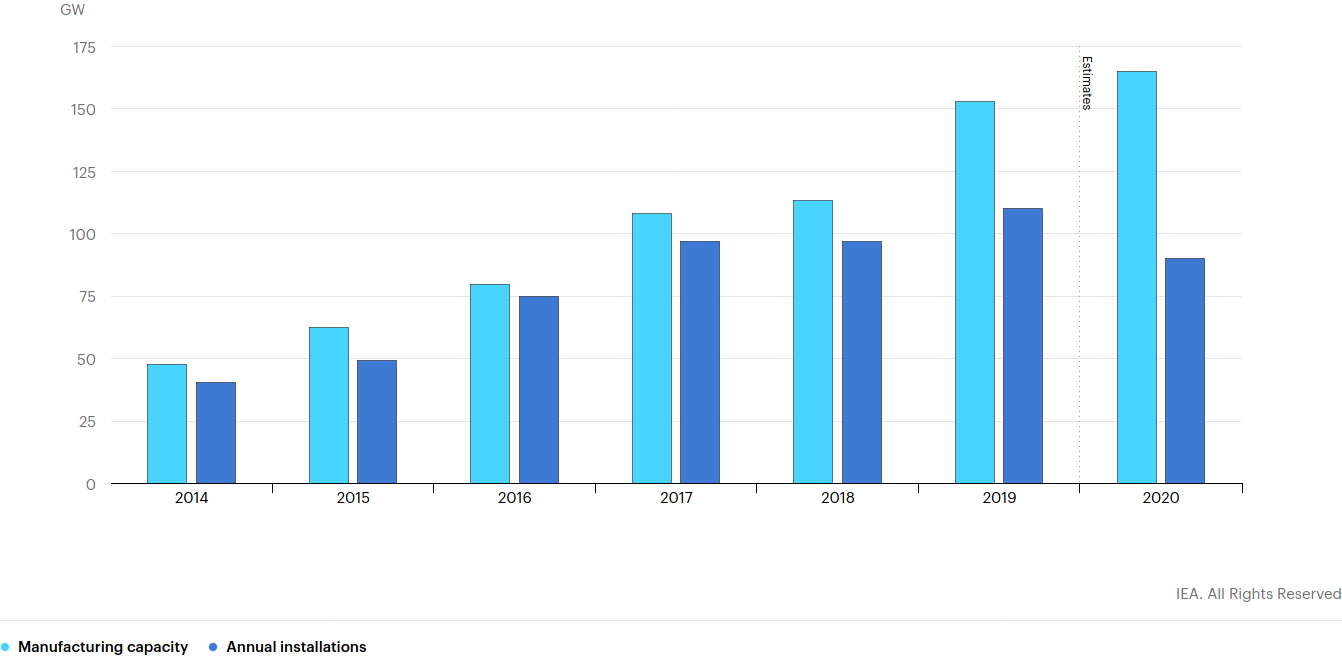
\includegraphics[width=\textwidth]{resources/ieapv.png}
    \caption{Fabrication et demande des modules solaires photovoltaïques, 2014-2020. Source: IEA analysis based on Paula Mints (2020), The Solar Flare, SVP Market Research, San Francisco, CA \cite{iea2020}}
    \label{fig:ieapv}
  \end{center}
\end{figure}
\begin{figure}
  \begin{center}
    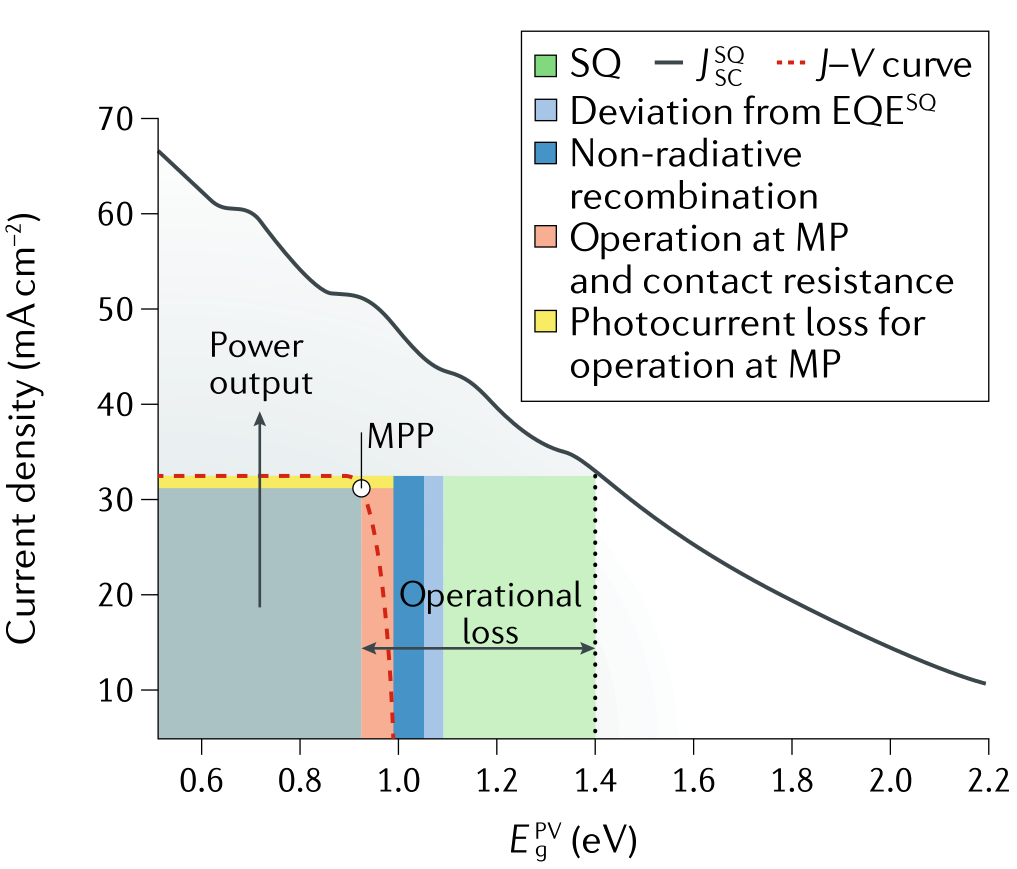
\includegraphics[width=0.5\textwidth]{resources/natsq.png}
    \caption{Différence entre le formalisme de SQ et une cellule réelle. Le photo-courant maximal CC à la limite de Schockley-Queisser est tracé en fonction du gap ($E_{g}^{PV}$). La ligne pointillée en rouge indique la caractéristique J-V de la cellule \cite{nayak2019}}
    \label{fig:natsq}
  \end{center}
\end{figure}

  \chapter{Modèles à circuits électriques pour les cellules PV}

\section{Généralités}

Fondamentalement, les cellules PV se composent de deux couches de semi-conducteurs à dopages différents, la jonction de ces deux couches étant exposée à la lumière incidente. En effet, les électrons dans la bande de conduction sont capables d'être transférés vers la bande de valence tant que l'énergie du photon incident $E = h \nu$ est supérieure à la largeur de la bande interdite $E_g = E_c - E_v$. Toute l'architecture d'une cellule quelconque vise à profiter le plus que possible de la différence de tension engendrée par les excitons séparés par le champ électrique dans la zone de déplétion (ou zone de charge d'espace) (figure \ref{fig:pn}). Par exemple, les contacts supérieurs sont des oxydes transparents conductifs (dit couche fenêtre) pour laisser passer le plus grand nombre de photons possible vers la couche absorbante de la cellule. Pour quelques cellule en couche mince, le contact arrière se compose d'une couche réfléchissante (ZnO et Ag ou Al) qui renvoie la lumière vers la couche absorbante pour minimiser davantage les pertes en lumière transmise \cite{Chopra2004}.\\

\begin{figure}
  \begin{center}
    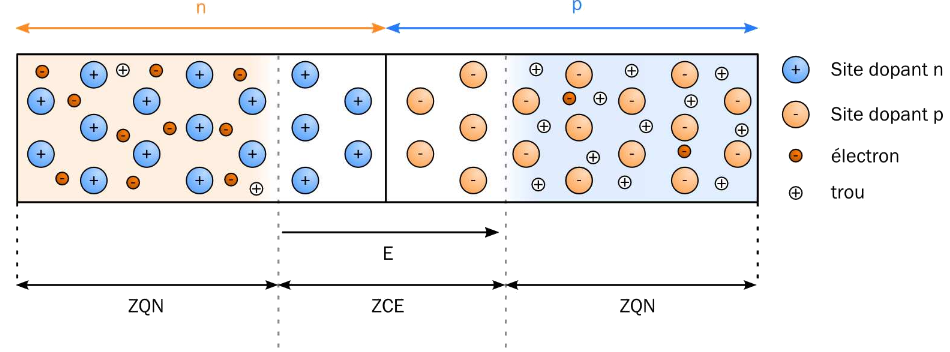
\includegraphics[width=.7\textwidth]{resources/pn.PNG}
    \caption{Schéma d'une jonction PN représentant : la zone de charge d'espace
(ZCE), les zones quasi-neutres (ZQN), les différents porteurs de charge, les sites dopants et le champ électrique E - Roger, 2013 \cite{Roger2013}.}
    \label{fig:pn}
  \end{center}
\end{figure}  

En fait, le comportement électrique d'un telle cellule en l'absence de la lumière est identique à celui d'une diode PN classique dont la caractéristique est décrite par l'équation de Shockley (équation \ref{eq:shockley}). Dans cette formule, le $I_0$ est le courant de saturation de la diode, $q$ la charge élémentaire $e^{-}$, $a$ le facteur d'idéalité, $k$ la constante de Boltzmann et $T$ la température de la cellule. Parfois on utilise la notion de \textit{voltage thermique}: $V_t = \frac{kT}{q}$.

\begin{equation}
\label{eq:shockley}
  I_D = I_0 \bigg[e^{\big(\frac{qV}{akT}\big)} - 1\bigg]
\end{equation}

Bien que ces modèles d'éléments localisé sont efficaces et précis pour les cellules de première génération et celles en couches minces, il existe aujourd'hui plusieurs technologies émergentes qui n'utilisent pas le champs électrique de la zone de déplétion pour la séparation des charges, et utilisent d'autre mécanismes et sources de champ électrique comme par la divergence positive de la polarisation $\nabla \cdot \bf{P} \neq 0$ qui crée un déséquilibre de charges aux parois de domaines à polarisation différentes sein des matériaux ferroélectriques \cite{Huang2010}. Pour ce genre de technologies, il est toujours difficile de concevoir un modèle de diode pour simuler le comportement complexe de ces cellules.

%\subsection{Modèles à simple diode}

Avec la présence de la lumière, les photons assez énergétique permettent la création des paires électron-trous qui, à leur tour, créent une différence de potentiel à travers la jonction. Une partie de ces porteurs de charge se recombine, mais l'autre se diffuse à travers les contacts de la cellule, ce qui donne naissance à un \textit{photo-courant} $I_{PV}$ (ou $I_L$) dont la valeur dépend de l'intensité de la lumière incidente.\\
En ajoutant le photo-courant $I_{PV}$ à l'équation de Shockley \ref{eq:idealmodeleq}, on retrouve un modèle élémentaire qui décrit une cellule idéale, composé d'une source de courant connectée à une diode en parallèle (figure \ref{fig:idealcell}). Évidemment ce modèle est complètement décrit par trois paramètres: \textit{(i)} Le photo-courant $I_{PV}$, \textit{(ii)} le facteur d'idéalité de la diode $a$ et \textit{(iii)} son courant de saturation $I_0$. 
\begin{equation}
\label{eq:idealmodeleq}
  I = I_{PV} - I_0 \bigg[e^{\big(\frac{qV}{akT}\big)} - 1\bigg]
\end{equation}

On voit dans la figure \ref{fig:idealcell}.b que la courbe caractéristique connue de la cellule se forme par une translation verticale par $I_{PV}$ d'une part, et de la forme exponentielle de la diode de l'autre. Le facteur la courbure dans la région du point de puissance maximale est déterminée par le facteur d'idéalité de la diode.

\begin{figure*}[t!]
  \centering
  \begin{subfigure}[t]{0.3\textwidth}
      \centering
      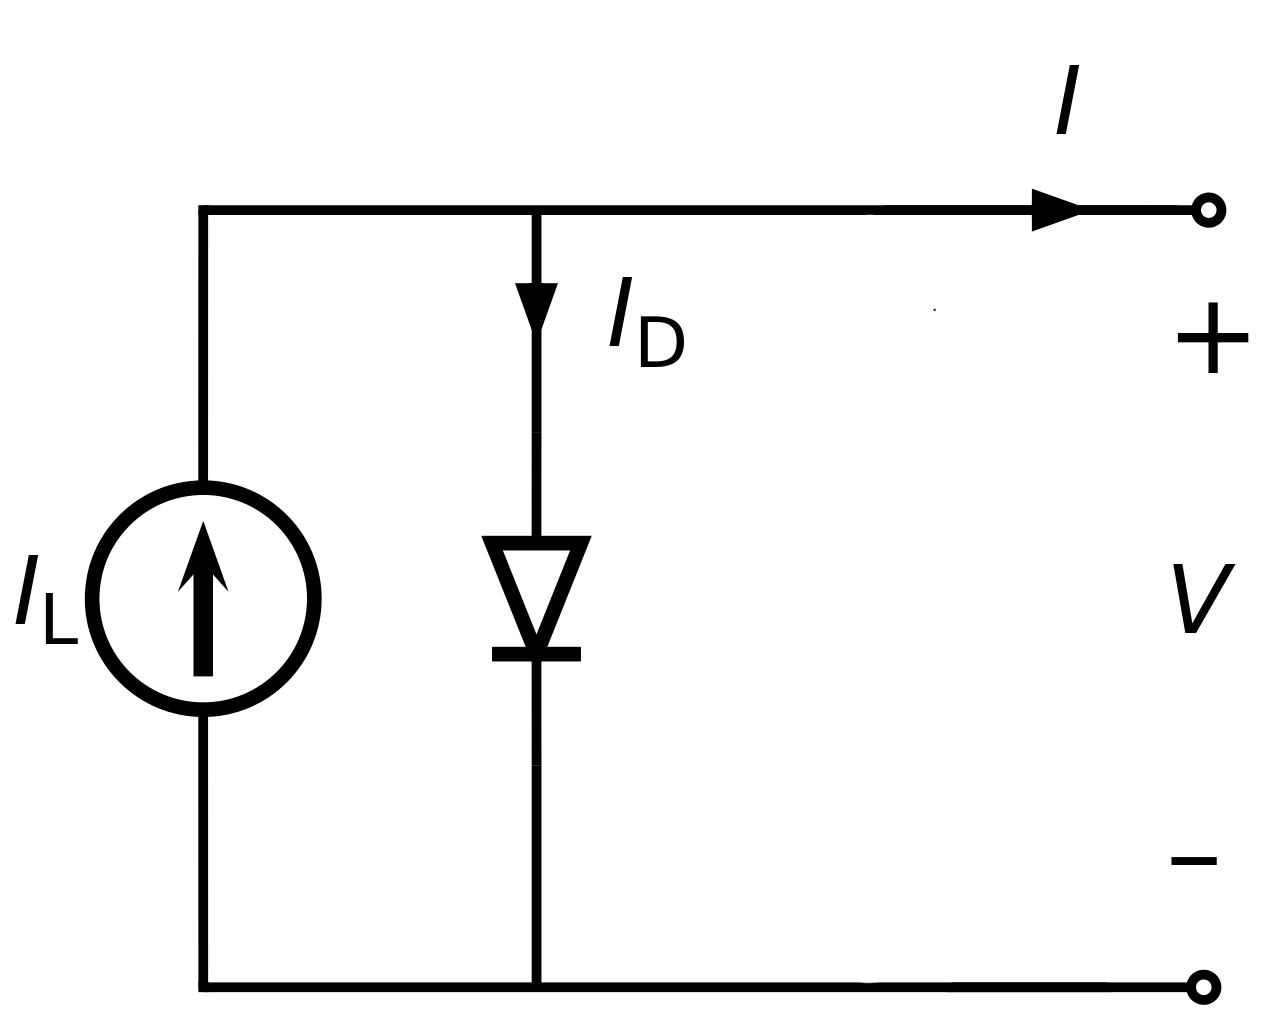
\includegraphics[width=\textwidth]{resources/idealcell.png}
      \caption{Modèle d'une cellule idéale}
  \end{subfigure}
  ~
  \begin{subfigure}[t]{0.65\textwidth}
      \centering
      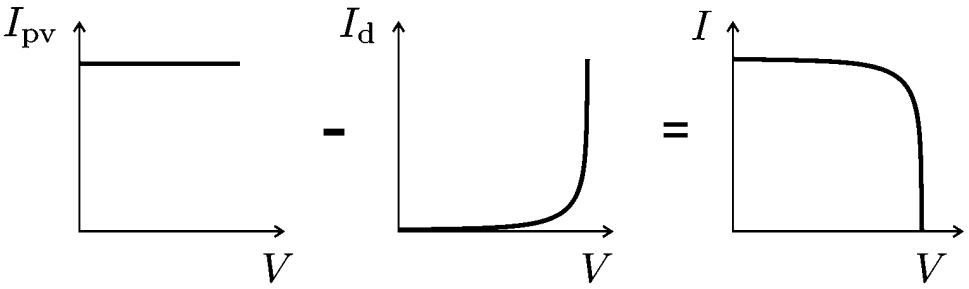
\includegraphics[width=\textwidth]{resources/superp.png}
      \caption{Le courant I est la superposition de $I_{PV}$ et de $I_D$ \cite{Villalva2009}}
  \end{subfigure}
  \caption{Modèle idéal d'une cellule PV}
  \label{fig:idealcell}
\end{figure*}

\section{Les modèles simple diode $R_S$ et $R_P$}
Le modèle idéal précèdent est utile pour éclaircir le concept de la modélisation par circuits d'éléments localisés. Dans la pratique, et pour plus de précision, il est nécessaire de considérer les pertes ohmique de la cellule dans le matériau semi-conducteur utilisé et dans les contacts des électrodes. La manière la plus directe de modéliser ces phénomènes est de tout simplement ajouter une résistance en série $R_S$ au circuit idéal. Ceci nous laisse avec la relation modifiée \ref{eq:singlers} du modèle dit \textit{"simple diode-$R_S$"} qui a besoin de 4 paramètres pour une description complète: $I_{PV}$, $a$, $I_0$ et $R_S$.\\
L'une des limites de ce modèle provient de son imprécision lorsque la cellule subit des variations négligeables de température. L'insertion d'une résistance shunt permet d'améliorer la sensibilité du modèle aux variations de température, et en même temps de considérer tout courant de fuite pouvant traverser la jonction \cite{Chin2015b}. On se retrouve cette fois avec les 5 paramètres du modèle dit \textit{"simple diode-$R_P$"} ou tout simplement \textit{"simple diode"}: $I_0$, $I_{PV}$, $a$, $R_s$ et $R_P$. La relation entre ces paramètres est décrite par l'équation \ref{eq:single}. Ce modèle offre un compromis entre la simplicité et la précision et par conséquent est très largement testé et utilisé dans la littérature \cite{Carrero2007}. Le diagramme du circuit de ce modèle est présenté dans la figure \ref{fig:single}.

\begin{equation}
  \label{eq:singlers}
  I = I_{PV} - I_0 \bigg[e^{\big(\frac{q(V + RS)}{akT}\big)} - 1\bigg]
\end{equation}

\begin{equation}
  \label{eq:single}
  I = I_{PV} - I_0 \bigg[e^{\big(\frac{q(V + RS)}{akT}\big)} - 1\bigg] - \frac{V + I R_S}{R_P}
\end{equation}

\begin{figure}
  \begin{center}
    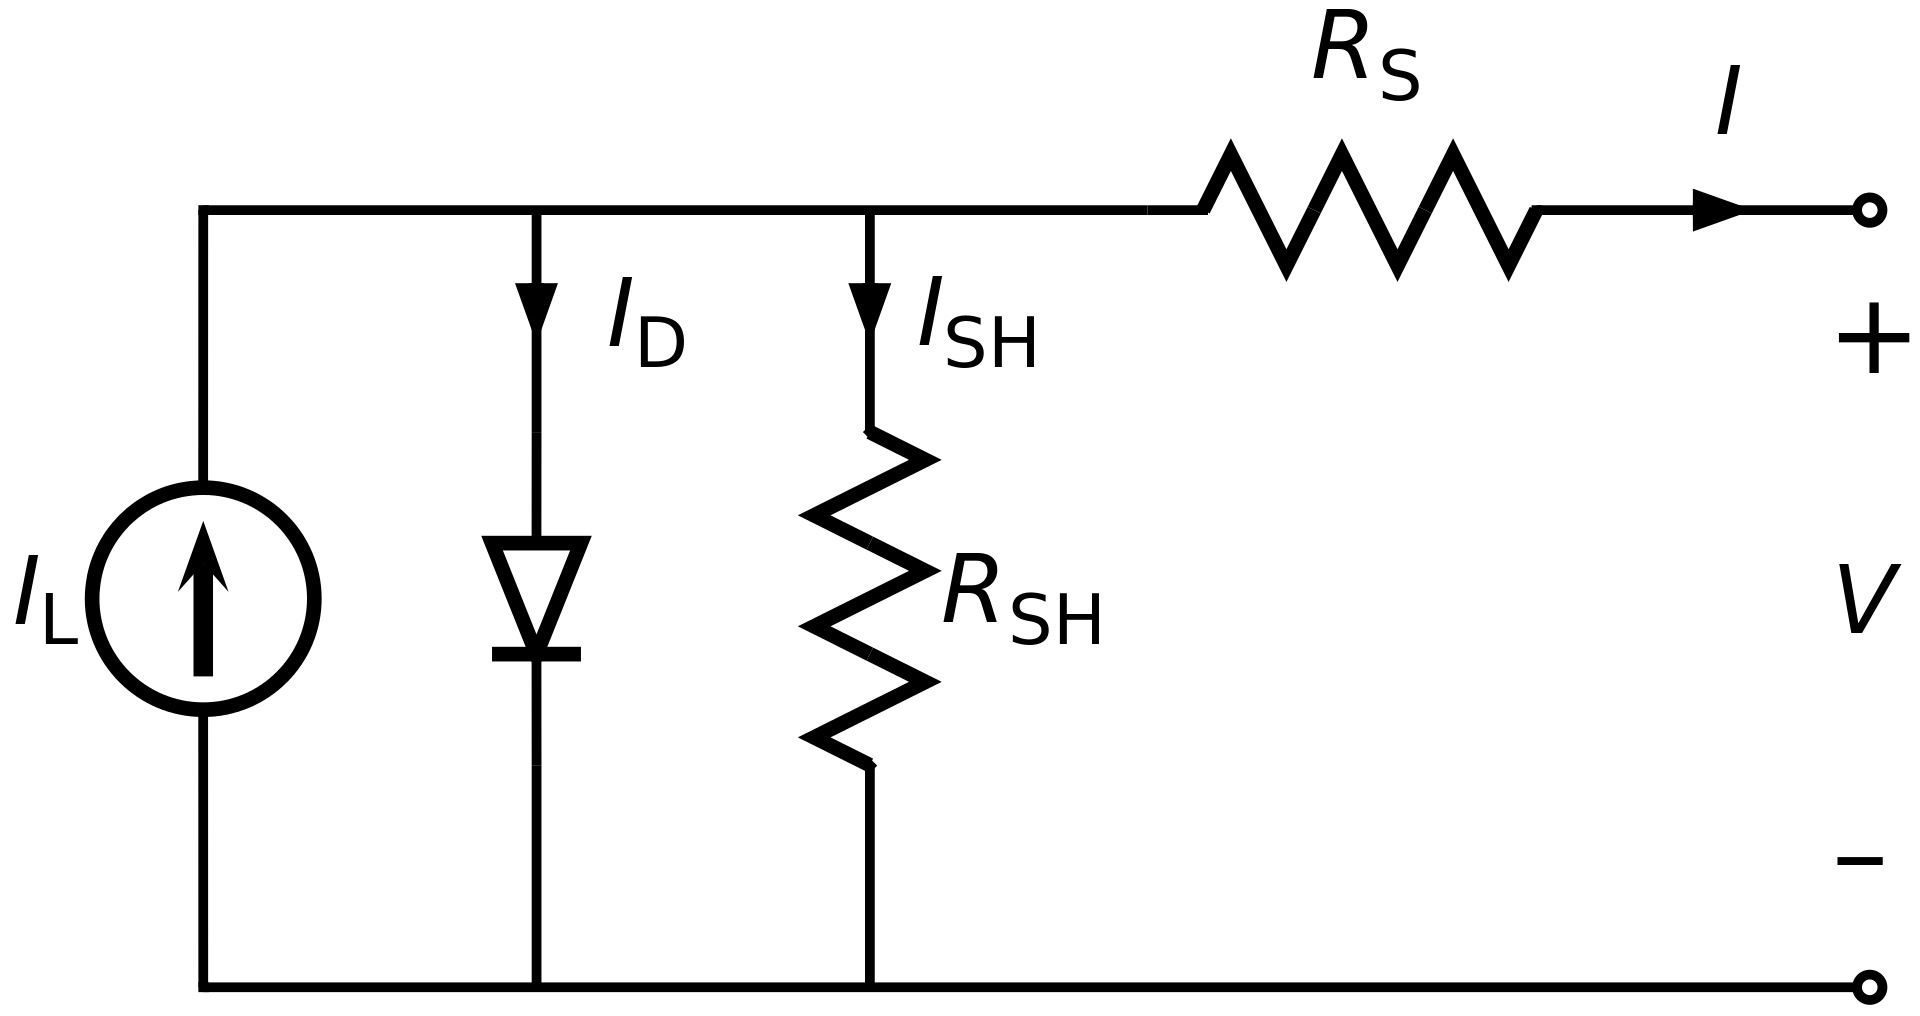
\includegraphics[width=.5\textwidth]{resources/eqcirc.png}
    \caption{Modèle Simple Diode}
    \label{fig:single}
  \end{center}
\end{figure}

\section{Modèle double diode}

Jusque là on a graduellement amélioré la performance et la précision des modèles de cellules PV en considérant de plus en plus de phénomènes physique qui se produisent dans la cellule (pertes ohmiques, effets des variations de température et courants de fuites). Un phénomène potentiellement influent qui n'est pas considéré par le modèle simple diode est celui des recombinaisons. Comme son nom l'indique, le modèle \textit{"double diodes"} (figure \ref{fig:doublediode} n'est que qu'un modèle simple diode auquel on ajoute une autre diode en shunt pour mieux modéliser les effets de recombinaisons surtout aux conditions d'illumination faible \cite{Chin2015b}.\\
Il est évident que l'addition d'une autre diode complique considérablement le modèle et on se retrouve avec deux paramètres supplémentaires ($I_{PV}$, $I_{01}$, $I_{02}$, $a1$, $a2$, $R_S$ et $R_P$). Toutefois, dans les cas où la complexité des calculs associés n'est pas contraignante, la précision de se modèle est supérieure. L'équation \ref{eq:doublediode} décrit la relation entre les 7 paramètres du modèle.
\begin{equation}
  \label{eq:doublediode}
  I = I_{PV} - I_{01} \bigg[e^{\big(\frac{q(V + RS)}{a_1kT}\big)} - 1\bigg] - I_{02} \bigg[e^{\big(\frac{q(V + RS)}{a_2kT}\big)} - 1\bigg] - \frac{V + I R_S}{R_P}
\end{equation}
\begin{figure}
  \begin{center}
    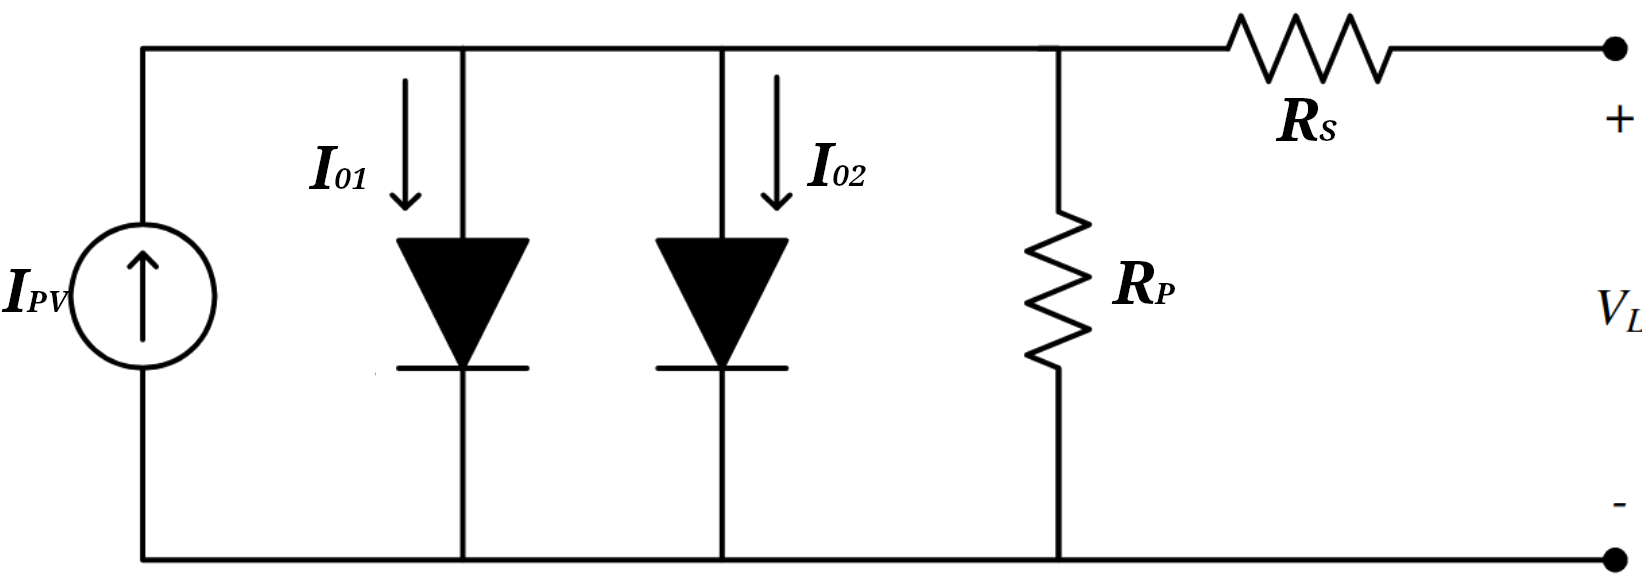
\includegraphics[width=.5\textwidth]{resources/doublediode.png}
    \caption{Le modèle double diode}
    \label{fig:doublediode}
  \end{center}
\end{figure}

\section{Influence des paramètres des modèles}

\section{Estimation des paramètres}

Les paramètres (soit les valeurs des éléments localisés des circuits) représentent une description complète du modèle et une bonne estimation de leurs valeurs est essentielle avant leur application. On utilise souvent les données des data-sheets offertes par les fabricants des cellules et modules PV. Ces données couvrent les points clés de la caractéristique I-V (court-circuit, circuit ouvert et puissance maximale). Les méthodes analytiques tendent à utiliser ces informations en plus de quelques expressions comme la pente de la courbe aux points clés pour déterminer les résistances en shunt $R_P$ et en série $R_S$. On trouve souvent aussi des simplifications comme le fait de considérer que seuls les $I_{PV}$ et $I_0$ sont significativement influents sur la caractéristique \cite{Ciulla2014}.
Dans le modèle simple diode contenant les 5 paramètres $I_{PV}$, $I_0$, $a$, $R_S$ et $R_P$, il est très courant de tout simplement négliger $I_0$ devant $I_{PV}$ au point court circuit, et par conséquent considérer que $I_{PV} = I_{CC}$ (La valeur de $I_0$ est ensuite extraite des conditions circuit ouvert) \cite{Villalva2009,Ciulla2014,Tsai2008}. En ce qui concerne $a$, $R_S$ et $R_P$, on a besoin de davantage d'équations. Généralement, les chercheurs utilisent soit les dérivées de la caractéristique aux points clés, soit des expressions analytiques des coefficients de température le liant avec les paramètres.\\
Le problème étant de nature non-linéaire, les techniques d'optimisation avec des capabilités de recherche globales dans l'espace de recherche s'offrent comme alternative. La précision de ces techniques dépends évidemment de la fonction objectif considérée, des conditions initiales et de la nature de l'algorithme lui-même \cite{Easwarakhanthan1986b, El-Naggar2012, DaCosta2010}. Les techniques de calcul souple et les algorithmes évolutionnistes ont susciter beaucoup d'intérêt récemment dans la littérature dans le but d'estimer les paramètres des cellules PV. Des techniques de réseaux de neurones artificiels [94, 98, 94], logique floue [109, 110, 111], algorithme génétique [76, 77 113], optimisation par essaims particulaires (Particle Swarm Optimization) [81, 115, 83] et évolution différentielle \cite{DaCosta2010, Ishaque2012, Gong2013} ont été utilisées. Par contre elles ne sont pas utilisées par les simulateurs PV, qui sont contraints par des critères de consistance et de temps de calcul, à cause de leurs nature stochastique. Ceci dit, elles sont très utiles lorsqu'il y a un besoin de précision sur les paramètres pour servir à l'optimisation du processus de fabrication ou pour l'étude de dégradation des cellules \cite{Ikegami2001,Balzani2005}. Dans les chapitres suivants nous allons présenter et analyser une méthode utilisant l'algorithme d'évolution différentielle qui est relativement récente en la comparant avec d'autre algorithmes similaires.

  \chapter{Évolution Différentielle}

\section{Introduction}

\section{Description de l'algorithme}

\section{Application aux modèles simple et double diodes}

\section{Métaheuristique}

  \chapter{Évolution Différentielle sur les circuits simple et double diodes}

\section{Introduction}
Maintenant que nous avons abordé les modèles à diodes et l'Évolution Différentielle indépendemment l'un de l'autre, dans ce chapitre nous allons appliquer l'ED \nomenclature{ED}{Évolution Differentielle (\textit{Differential Evolution})} sur les modèles pour estimer les valeurs des paramètres en utilisant les données expérimentales standards de la littérature. En ce qui concerne l'implémentation pratique de cette technique, on utilise le langage de programmation \textit{Python}. On fait appel a quelques bibliothèques scientifiques de Python pour fournir les outils mathématiques requis par la méthode. A partir d'ici nous allons fournir des petits extraits de code pertinents à la discussion qui montrent la manière d'implémenter les étapes de la méthode. Pour des raisons de clarté ce ne sont pas des extraits complètement fidèles au code utilisé en réalité. Le code complet et non modifié est disponible comme annexe à la fin de ce document. 

\section{Fonction W de Lambert}
Les méthodes évolutionnaires dépendent d'une fonction objectif qu'il faut minimiser, pour sélectionner les meilleures solutions dans une population. Dans notre cas, la fonction objectif est la \textit{RMSE} \nomenclature{RMSE}{Racine de l'erreur quadratique moyenne (\textit{Root Mean Squared Error})} et elle quantifie la différence entre la courbe caractéristique du modèle et les données expérimentales. Cependant, chaque fois qu'un vecteur solution $\vec{V}$ (formules \ref{eq:vsol}) est généré, il faut pouvoir recréer la courbe I-V associée pour permettre à la fonction objectif de calculer la RMSE.
\begin{equation}
  \label{eq:vsol}
  \vec{V}_{\text{simple diode}} = 
  \begin{bmatrix}
    R_s\\
    R_{p}\\
    a\\
    I_0\\
    I_{PV}
  \end{bmatrix},
  \quad
  \vec{V}_{\text{double diode}} = 
  \begin{bmatrix}
    R_s\\
    R_{p}\\
    a_1\\
    a_2\\
    I_{01}\\
    I_{02}\\
    I_{PV}
  \end{bmatrix}
\end{equation}
On pourrait implémenter la fonction objectif en code de la manière suivante:
\begin{python}
# Cette fonction prend un vecteur solution et les points IV experimentaux comme arguments
def objf(vecteur, exp_v, exp_i):
    # Penalisons le vecteur si les valeurs sont non-physiques
    rs, rp = vecteur[0], vecteur[1]
    if rs < 0 or rp < 0:
        return 100 # Valeur fitness large
    ical = i_from_vect(vector, exp_vol) # Une fonction donnant la caracteristique IV de "vector"
    erreur = ical - exp_i
    return np.sqrt(np.mean(erreur ** 2)) # RMSE  
\end{python}

Les équations de modèles simple et double diode (équations \ref{eq:single}, \ref{eq:doublediode}, respectivement) sont transcendantes, il est donc impossible d'extraire directement le courant à partir de la tension et des paramètres (Le courant $I$ figure simultanément dans le premier membre et dans l'exponentiel du second). Ainsi, il n'est pas trivial de remplir la fonction de \pyth{i_from_vect(vector, exp_vol)}. Plusieurs méthodes on été utilisées initialement avec des approches d'approximation analytique ou itérative \cite{Shur1991,AbuelmaAtti1992,Datta1992}. Ces méthodes sont approximatives mais permettent de trouver la solution explicitement avec des fonctions élémentaires (Développement Taylor par exemple). Dans notre cas, on fait recours à la méthode de Jain et Kapoor (2004) \cite{Jain2004, Lun2015} qui utilisent la fonction W de Lambert pour une solution analytique exacte de ces équations.

\subsection{Définition}
La "\textit{fonction W}" de Lambert est définie comme l'inverse de la fonction $w \rightarrow f(w) =  w e^w$, où $w = W_k(z)\ |\ z \in \mathbb{C}$. La fonction $f$ n'étant pas surjective, la fonction $W_k(z)$ est donc \textit{multivaluée} et comprends plusieurs branches indexées par $k$ ($W_0$ est choisie comme branche principale). Si $x \in \mathbb{R}$, donc pour $-1/e \leq x < 0$, il existe deux valeurs réelles possible de $W(x)$ (figure \ref{fig:lambertw}).

\begin{figure} 
  \begin{center}
    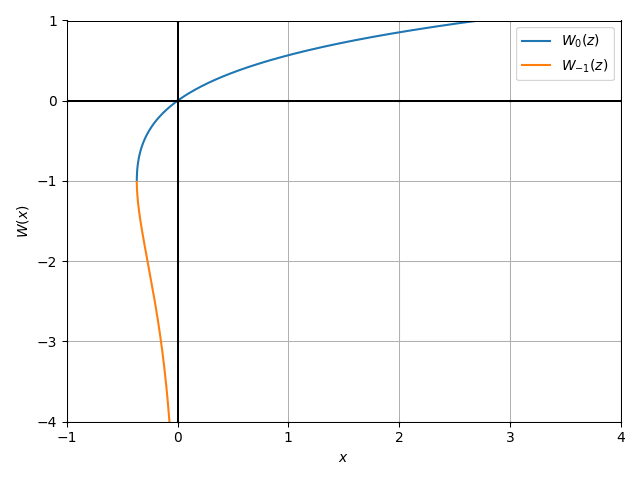
\includegraphics[width=.6\textwidth]{resources/lambertw.png}
    \caption{Les deux branches réelles de $W(x)$ lorsque $x$ est réel}
    \label{fig:lambertw}
  \end{center}
\end{figure}

\subsection{Évaluation de la fonction $W$}

Le fait qu'il n'existe pas de fonctions mathématiques élémentaires donnant explicitement $W(z)$ est remédié par l'existence de plusieurs \textit{algorithmes de recherche des zéros} permettant le calcul de les valeurs de n'importe quelle branche de la fonction $W$. Dans notre cas spécifique, la bibliothèque scientifique \textit{scipy} de Python fournit une fonction W implémentée par l'itération de Halley qui est un exemple d'une méthode de classe "Householder". La méthode de Halley a été appliquée à la fonction $W$  par Corless et al. \cite{Corless1996} donnant:
\begin{equation}
  \label{eq:halley}
  w_{j+1} = w_j - \frac{w_j e^{w_j} - z}{e^{w_j}(w_j + 1) - \frac{(w_j + 2)(w_j e^{w_j} - z)}{2w_j + 2}}
\end{equation}

Un exemple basique de l'utilisation de cette méthode en Python est le suivant:

\begin{python}[basicstyle=\tiny]
import numpy as np 
from scipy.special import lambertw # scipy fournit la fonction W

z = np.linspace(-1/np.e, 3, 1000) # evaluons W entre -1/e et 3
w0 = lambertw(z, 0) # choisir la branche principale
\end{python}

\subsection{Résolution de modèles simple et double diode par la fonction W}
De la définition de la fonction W, la solution d'une équation $xe^x = a$ est $x = W(a)$. En effectuent des manipulations algébriques élémentaires sur le modèle simple diode (equation \ref{eq:single}), Jain et Kapoor ont montré que l'expression explicite du courant en fonction des paramètres et de la tension est:
\begin{equation}
  \label{eq:lambertwsingle}
  I = \frac{R_{sh}(I_0 + I_{PV}) - V}{R_s + R_{sh}} - \frac{W\left(\frac{R_s I_0 R_{sh}}{a V_{th}(R_s + R_{sh})}e^{\left(\frac{R_{sh}(R_s I_{PV} + R_s I_0 + V)}{a V_{th} (R_s + R_{sh})}\right)}\right)aV_{th}}{R_s}
\end{equation}
On remarque bien que le second membre ne contient nul part un terme de courant $I$. Il faut noter aussi que le terme de la fonction $W$ est sous risque d'un dépassement et de retourner de valeurs infinies. Pour des raisons de stabilité numérique on utilise la notion de \textit{Conductance Shunt}: $C_{sh} = \frac{1}{R_{sh}}$ car cette résistance prend souvent de valeurs $\gg 1$ ce qui entraîne un risque de divergence des calculs. On trouve souvent des valeurs larges de résistance shunt, ce qui explique l'existence dans la littérature de plusieurs modèles utilisant la simplification $R_{sh} = + \infty$. Avec la substitution de la conductance shunt, si $R_{sh}\rightarrow\infty$ alors $C_{sh} \rightarrow 0$ ce qui assure la stabilité du calcul numérique.

Le modèle double diodes (équation \ref{eq:doublediode}) contient un terme exponentiel pour chaque diode. De la même manière que Jain et Kapoor on retrouve explicitement l'expression du courant avec deux termes de la fonction $W$ (equation \ref{eq:lambertwdouble}).
\begin{equation}
  \label{eq:lambertwdouble}
  \begin{split}
    I &= \frac{R_{sh} (I_{01} + I_{02} + I_{PV}) - V}{R_s + R_{sh}}\\ 
    &- \frac{a_1}{2 R_s} W\left( \frac{R_s R_{sh}(I_{01} + I_{02})}{a_1 (R_s + R_{sh})}e^{\left(\frac{R_{sh}(R_s I_{PV} + R_s I_{01} + R_s I_{02} + V)}{a_1 (R_s + R_{sh})}\right)}\right)\\ 
    &- \frac{a_2}{2 R_s} W\left( \frac{R_s R_{sh}(I_{01} + I_{02})}{a_1 (R_s + R_{sh})}e^{\left(\frac{R_{sh}(R_s I_{PV} + R_s I_{01} + R_s I_{02} + V)}{a_2 (R_s + R_{sh})}\right)}\right)
  \end{split}
\end{equation}

\section{Résultats}

\subsection{Configuration de l'Évolution Différentielle}
\nomenclature{$F$}{Facteur de mutation}
\nomenclature{$CR$}{Taux de croisement}
\nomenclature{$N_P$}{Taille de la population}
%\nomenclature{$Gen_{max}$}{Nombre maximal de générations}
\nomenclature{$D$}{Dimensions de l'espace de recherche}
Pour appliquer l'Évolution Différentielle avec succès sur les modèles à diodes, il faut savoir choisir les bonnes valeurs de paramètres de contrôle $CR, F \text{et}\  N_P$. Il n'existe pas de règle stricte mais Storn et Price \cite{Price2005} donnent quelques indications. En ce qui concerne le facteur de mutation $F$, les valeurs $F \geq 1$ ne sont pas fiables et souvent convergent très lentement par rapport aux $F < 1$. Cependant, Zaharie (2002) \cite{Zaharie2002} constate une borne inférieure de $F > 0.4$. Puisque l'opération de \textit{sélection} tend à réduire la diversité dans la population, le rôle de la \textit{mutation} et de balancer cette pression exercée sur la population et tend à augmenter la diversité. Si $F$ est trop petit, l'ED peut converger même avec l'absence de la pression sélective. En ce qui concerne le taux de croisement $CR$, Salomon (1996) \cite{Salomon1996} a démontré les limites d'un $CR$ trop petit et par conséquent Storn et Price recommandent des valeurs de $CR$ proche de $1$. Reste à choisir la taille de la population $N_P$, généralement $10D \leq N_P \leq 20D$ est recommandé mais dans notre cas on optera à $N_P = 100$.

\subsection{Cas 1: Cellule 57-mm de RTC France}

Ce premier cas d'étude concerne la cellule en silicium de RTC France avec un diamètre de 57 mm qui a été très largement étudiée dans la littérature. Sa courbe caractéristique a été mesurée dans des conditions de température $T = \SI{33}{\celsius}$ et irradiance solaire $\SI{1000}{\watt\per\square\meter}$ et comprend 26 points expérimentaux (figure \ref{fig:RTCexp}). Figure \ref{fig:RTCres}.a montre que la caractéristique expérimentale et calculée par l'ED sont graphiquement quasi-identiques. Figure \ref{fig:RTCres}.b montre l'évolution de la moyenne des valeurs de fitness des vecteurs évalués par la fonction objectif dans chaque génération consécutive. On constate que dès la 50\textsuperscript{ème} génération, l'ED a pratiquement déjà convergé.

Le tableau \ref{tab:RTCres} présente une comparaison entre l'ED et d'autre méthodes appliquées à la cellule RTC France. On constate que les valeurs retrouvées par l'ED sont assez proches de celles des autres travaux. En effet, l'ED parvient à une erreur RMSE de \num{7.7692e-04} qui est supérieure aux autres techniques similaire comme les essaims particulaires \cite{Hamid2016}, l'algorithme des colonies d'abeilles artificielles \cite{Oliva2014} et l'ED à trois points \cite{Chin2019}. Les résultats les moins précis sont ceux de la méthode de Newton à moindres carrés \cite{Easwarakhanthan1986}.

\begin{table}
  \caption{Bornes utilisées de l'espace de recherche pour le modèle simple diode}
  \label{tab:singleboundaries}

  \begin{center}
    \begin{tabular*}{.7\textwidth}{l@{\extracolsep{\fill}}cc}
       \hline
       \textbf{Paramètre} & \textbf{Borne inférieure} & \textbf{Borne supérieure}   \\
       \hline
       $R_s$    & 0 & 1 \\
       $R_{sh}$ & 2 & 100 \\
       $a$      & 1 & 2\\
       $I_0$    & \num{1e-07} & \num{1e-04} \\
       $I_{PV}$ & 0 & 10\\
       \hline
    \end{tabular*}
  \end{center}
\end{table}

\begin{figure}
  \begin{center}
    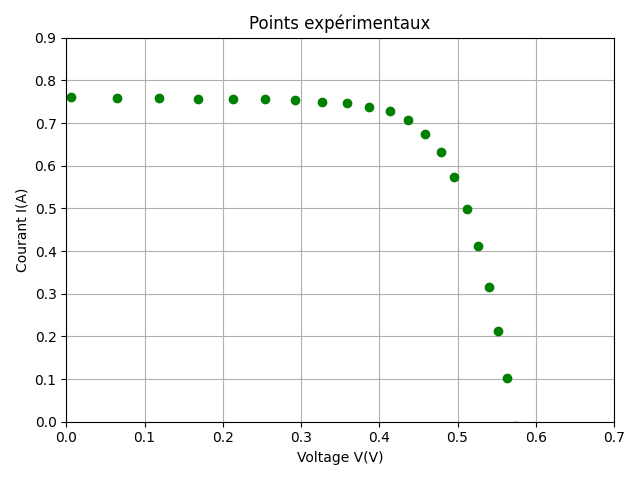
\includegraphics[width=0.6\textwidth]{resources/RTCFrance/exp.png}
    \caption{Données expérimentales de la caractéristique IV de la cellule RTC France mesurées à \SI{33}{\celsius}}
    \label{fig:RTCexp}
  \end{center}
\end{figure}

\begin{figure*}[t!]
    \centering
    \begin{subfigure}[b]{0.45\textwidth}
        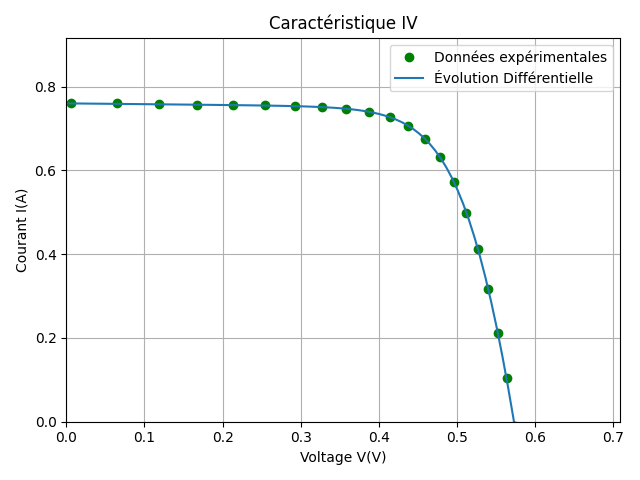
\includegraphics[width=\textwidth]{resources/RTCFrance/singled/iv.png}
        \caption{Comparaison entre la courbe expérimentale et la caractéristique calculée.}
    \end{subfigure}
    ~
    \begin{subfigure}[b]{0.45\textwidth}
        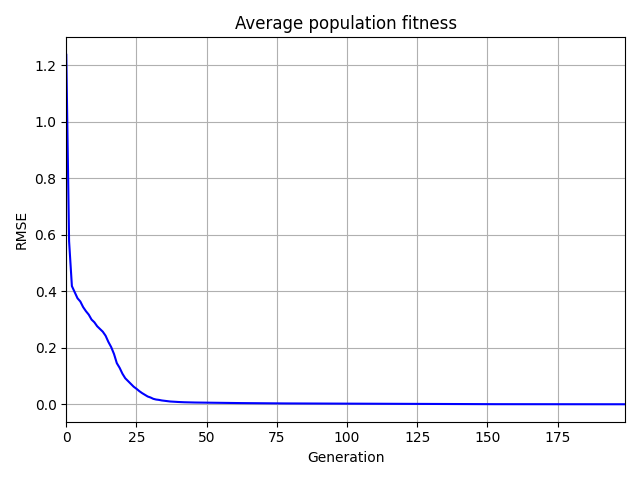
\includegraphics[width=\textwidth]{resources/RTCFrance/singled/fitness.png}
        \caption{Évolution de la valeur moyenne de fitness de chaque génération}
    \end{subfigure}
    \caption{Résultats de l'ED appliquée sur la cellule RTC France 57 mm.}
    \label{fig:RTCres}
\end{figure*}

\begin{table}
  \caption{Comparaison de l'ED avec d'autres méthodes dans la littérature}
  \label{tab:RTCres}

  \begin{center}
  \scriptsize
    \begin{tabular*}{\textwidth}{l@{\extracolsep{\fill}}cllllll }
       \hline
       Paramètres & Référence & $R_s$ (\si{\ohm}) & $R_{sh} (\si{\ohm})$ & $a $ & $I_0$ (\si{\micro\ampere}) & $I_{PV}$ (\si{\ampere}) & $RMSE$ \\
       \hline
       ED (simple diode) &                            & \num{0.0363} & \num{54.1134} & \num{1.4709} & \num{0.3209} & \num{0.7607} & \num{7.7692e-04}\\
       ED3P              & \cite{Chin2019}            & \num{0.0363} & \num{54.1924} & \num{1.4798} & \num{0.3191} & \num{0.7607} & \num{8.1291e-04}\\
       PSO               & \cite{Hamid2016}           & \num{0.0363} & \num{53.8550} & \num{1.4816} & \num{0.3245} & \num{0.7607} & \num{9.8606e-04}\\
       ABC               & \cite{Oliva2014}           & \num{0.0364} & \num{53.6433} & \num{1.4817} & \num{0.3251} & \num{0.7608} & \num{9.8620e-04}\\
       Newton            & \cite{Easwarakhanthan1986} & \num{0.0364} & \num{53.7634} & \num{1.4837} & \num{0.3223} & \num{0.7608} & \num{9.70e-03}  \\
       GA                & \cite{Oliva2014}           & \num{0.0299} & \num{42.3729} & \num{1.5751} & \num{0.8087} & \num{0.7619} & \num{1.90e-02}  \\
       \hline
    \end{tabular*}
  \end{center}
\end{table}

\nomenclature{$ED3P$}{Évolution différentielle à trois points}
\nomenclature{ABC}{Colonies d'abeilles artificielles (\textit{Artificial Bee Colony Optimization})}

\subsubsection{Modèle double diode}
En ce qui concerne le modèle double diode, les deux facteurs d'idéalité $a_1$ et $a_2$ ainsi que les courants de saturation $I_{01}$ et $I_{02}$ sont indépendants les uns les autres mais sont contraints dans les limites dans le tableau \ref{tab:doubledboundaries}. Les résultats de l'ED en double diode sont comparés avec ceux de quelques autres méthode dans le tableau \ref{tab:RTCresdouble}.
\begin{table}[H]
  \caption{Bornes de l'espace de recherche à 7 dimensions}
  \label{tab:doubledboundaries}

  \begin{center}
    \begin{tabular*}{.7\textwidth}{l@{\extracolsep{\fill}}cc}
      \hline
      \textbf{Paramètre} & \textbf{Borne inférieure} & \textbf{Borne Supérieure}\\
      \hline
      $R_s$    & 0 & 1 \\
      $R_{sh}$ & 2 & 100 \\
      $a_1$    & 1 & 2\\
      $a_2$    & 1 & 2\\
      $I_{01}$ & \num{1e-07} & \num{1e-04} \\
      $I_{02}$ & \num{1e-07} & \num{1e-04} \\
      $I_{PV}$ & 0 & 10\\
       \hline
    \end{tabular*}
  \end{center}
\end{table}

\begin{table}[H]
  \caption{Comparaison de l'ED avec d'autres méthodes dans la littérature}
  \label{tab:RTCresdouble}

  \begin{center}
  \scriptsize
    \begin{tabular*}{\textwidth}{l@{\extracolsep{\fill}}cllllllll}
       \hline
       Paramètres & Référence & $R_s$ (\si{\ohm}) & $R_{sh} (\si{\ohm})$ & $a_1$ & $a_2$ & $I_{01}$ (\si{\ampere}) & $I_{02}$ (\si{\ampere}) & $I_{PV}$ (\si{\ampere}) & $RMSE$ \\
       \hline
       ED (double diode) &                            & \num{0.02061}   & \num{51.9345} & \num{1.87579} & \num{1.43602} & \num{4.2322e-07} 
                                                      & \num{1.8726e-07}& \num{0.76055} & \num{7.63e-04}   \\
       PSO               & \cite{Jordehi2016}         & \num{0.05861}   & \num{18.2106} & \num{1.00012} & \num{1.00091} & \num{2.8601e-10} 
                                                      & \num{1e-12}     & \num{0.7633}  & \num{8.1646e-03} \\
       GSA               & \cite{Jordehi2017}         & \num{0.02914}   & \num{51.116}  & \num{1.6087}  & \num{1.62889} & \num{6.60621e-7} 
                                                      & \num{4.55149e-7}& \num{0.76886} & \num{5.91958e-03}\\
       ABC               & \cite{Oliva2014}           & \num{0.0364}    & \num{53.7804} & \num{1.4495} & \num{1.4885} & \num{4.07e-08}
                                                      & \num{2.874e-07} & \num{0.7608}  & \num{9.861e-04}\\
       \hline
    \end{tabular*}
  \end{center}
\end{table}

\nomenclature{GSA}{Gravitational Search Algorithm}

\subsection{Cas 2: Module monocristallin Schutten Solar STM6-40/36}

Nous nous concernons dans ce deuxième cas d'étude du module monocristallin Schutten Solar STM6-40/36 composé de 36 cellules ($156\si{\milli\meter}\times 156\si{\milli\meter}$) en série. Les données expérimentales ont été prises à une température de 51\si{\celsius}. Une comparaison des résultats de l'ED avec d'autres méthodes est présentée dans le tableau \ref{tab:stm6}. La correspondance de la caractéristique calculée par l'ED aux points experimentaux est démontrée graphiquement dans la figure \ref{fig:STM6res}. Malgré la distribution irrégulière des points, l'ED arrive a produire une solution précise. Sa précision et de même ordre de grandeur que ED3P \cite{Chin2019} mais elle est supérieure aux techniques des colonies des abeilles artificielles (ABC) \cite{Oliva2014}, de sa version améliorée par Oliva et al. (CIABC) \cite{Oliva2017a} et Chaotic Whale Optimization Algorithm (CWOA) \cite{Oliva2017}.

\begin{figure*}[t!]
    \centering
    \begin{subfigure}[b]{0.45\textwidth}
        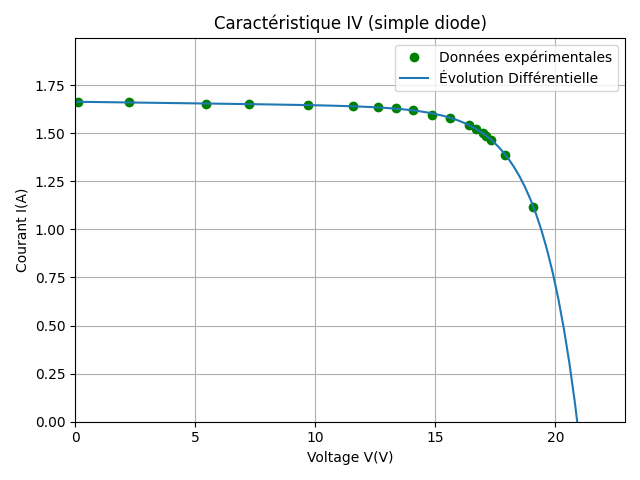
\includegraphics[width=\textwidth]{resources/STM6/singled/iv.png}
        \caption{Correspondence de l'ED aux données expérimentales. La distribution non-optimale des points n'entrave pas la convergence.}
    \end{subfigure}
    ~
    \begin{subfigure}[b]{0.45\textwidth}
        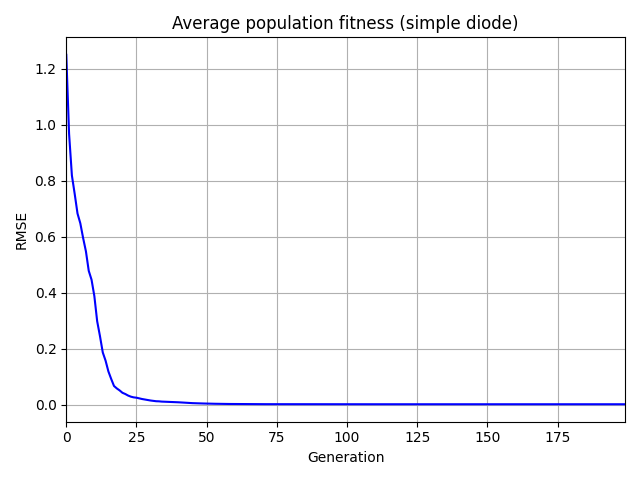
\includegraphics[width=\textwidth]{resources/STM6/singled/fitness.png}
        \caption{Évolution de la valeur moyenne de fitness de chaque génération. L'ED est convergeante dès la $50^{\text{ème}}$ itération.}
    \end{subfigure}
    \caption{Résultats de l'ED appliquée sur au module Schutten Solar STM6-40/36}
    \label{fig:STM6res}
\end{figure*}

\begin{table}
  \caption{Comparaison de l'ED avec d'autres méthodes dans la littérature sur le module STM6-40/36}
  \label{tab:stm6}

  \begin{center}
    \scriptsize
    \begin{tabular*}{\textwidth}{l@{\extracolsep{\fill}}cllllll}
      \hline
      Paramètres & Référence & $R_s$ (\si{\milli\ohm}) & $R_{sh} (\si{\ohm})$ & $a $ & $I_0$ (\si{\micro\ampere}) & $I_{PV}$ (\si{\ampere}) & $RMSE$ \\
      \hline
       ED (simple diode)  &                   & \num{0.2801} & \num{16.5854} & \num{1.5571} & \num{2.8049} & \num{1.6633} & \num{1.7721e-03}  \\
       ED3P               & \cite{Chin2019}   & \num{0.4186} & \num{16.7328} & \num{1.5656} & \num{2.7698} & \num{1.6632} & \num{1.7740e-03}  \\
       ABC                & \cite{Oliva2014}  & \num{4.99}   & \num{15.206}  & \num{1.4866} & \num{1.5}    & \num{1.6644} & \num{1.838e-03}   \\
       CIABC              & \cite{Oliva2017a} & \num{4.4}    & \num{15.617}  & \num{1.4976} & \num{1.6642} & \num{1.6760} & \num{1.819e-03}   \\
       CWOA               & \cite{Oliva2017}  & \num{5}      & \num{15.4}    & \num{1.5}    & \num{1.6338} & \num{1.7}    & \num{1.800e-03}   \\
       \hline
    \end{tabular*}
  \end{center}
\end{table}
\nomenclature{CIABC}{Chaotic Improved Artificial Bee Colony}
\nomenclature{CWOA}{Chaotic Whale Optimization Algorithm}

\subsubsection{Modèle double diode}

Les résultats de l'ED avec le modèle double diode sur le module STM6-40/36 sont présenté dans le tableau \ref{tab:STM6double} avec d'autres techniques tel quel les colonies d'abeilles artificielles et les essaims particulaires. Le tableau \ref{tab:stm6doublelimits} montre les bornes utilisées comme limites de l'espace de recherche. Notons la similarité des qualités des résultats du modèle simple et double diode.

\begin{table}[H]
  \caption{Comparaison de l'ED avec d'autres méthodes sur le module photovoltaïque STM6-40/36}
  \label{tab:STM6double}

  \begin{center}
  \scriptsize
    \begin{tabular*}{\textwidth}{l@{\extracolsep{\fill}}cllllllll}
       \hline
       Paramètres & Référence & $R_s$ (\si{\ohm}) & $R_{sh} (\si{\ohm})$ & $a_1$ & $a_2$ & $I_{01}$ (\si{\ampere}) & $I_{02}$ (\si{\ampere}) & $I_{PV}$ (\si{\ampere}) & $RMSE$ \\
       \hline
       ED (double diode) &                            & \num{0.0177}    & \num{16.7050}& \num{1.9049} & \num{1.52461}   & \num{1.006e-06} 
                                                      & \num{2.9858e-06}& \num{1.6633} & \num{1.7724e-03}   \\
       ELPSO             & \cite{RezaeeJordehi2018}   & \num{0.0138}    & \num{16.8580}& \num{1.8706} & \num{1.16648}   & \num{1.670e-08} 
                                                      & \num{6.21092e-6}& \num{1.6648} & \num{1.8307e-03}   \\
       ABC               & \cite{RezaeeJordehi2018}   & \num{0.03434}   & \num{26.0613}& \num{1.9851}  & \num{1.4687}** & \num{8.938e-6} 
                                                      & \num{1e-12}     & \num{1.66347}& \num{2.0538e-03}\\
       \hline
    \end{tabular*}
  \end{center}
\end{table}
\nomenclature{ELPSO}{Enhanced Leader Particle Swarm Optimization}

\begin{table}[H]
  \caption{Limites de l'espace de recherche pour l'ED double diode sur le module photovoltaïque STM6-40/36}
  \label{tab:stm6doublelimits}

  \begin{center}
    \begin{tabular*}{.7\textwidth}{l@{\extracolsep{\fill}}cc}
      \hline
      \textbf{Paramètre} & \textbf{Borne inférieure} & \textbf{Borne Supérieure}\\
      \hline
      $R_s$    & 0 & 1 \\
      $R_{sh}$ & 2 & 100 \\
      $a_1$    & 1 & 2\\
      $a_2$    & 1 & 2\\
      $I_{01}$ & \num{0} & \num{1e-04} \\
      $I_{02}$ & \num{0} & \num{1e-04} \\
      $I_{PV}$ & 0 & 10\\
      \hline
    \end{tabular*}
  \end{center}
\end{table}

\subsection{Analyse et cohérence de l'ED}

La performance supérieure démontrée par l'ED par rapport aux autres algorithmes provient probablement de ses capacités à la \textit{recherche globale}. L'existence d'une multitude de minimums locaux est demontrée dans la figure \ref{fig:neigh} où on a projeté l'espace de recherche 5-dimensionnel sur 2 dimensions au voisinage du minimum global. On fait varier le facteur d'idéalité $a$ et la résistance série $R_s$ dont le modèle est très sensible aux variations. Les trois autres paramètres $R_{sh}$, $I_0$ et $I_{PV}$ sont fixés sur les valeurs du minimum global retrouvé par l'ED comme dans le tableau \ref{tab:RTCres}.

\begin{figure}[H]
  \begin{center}
    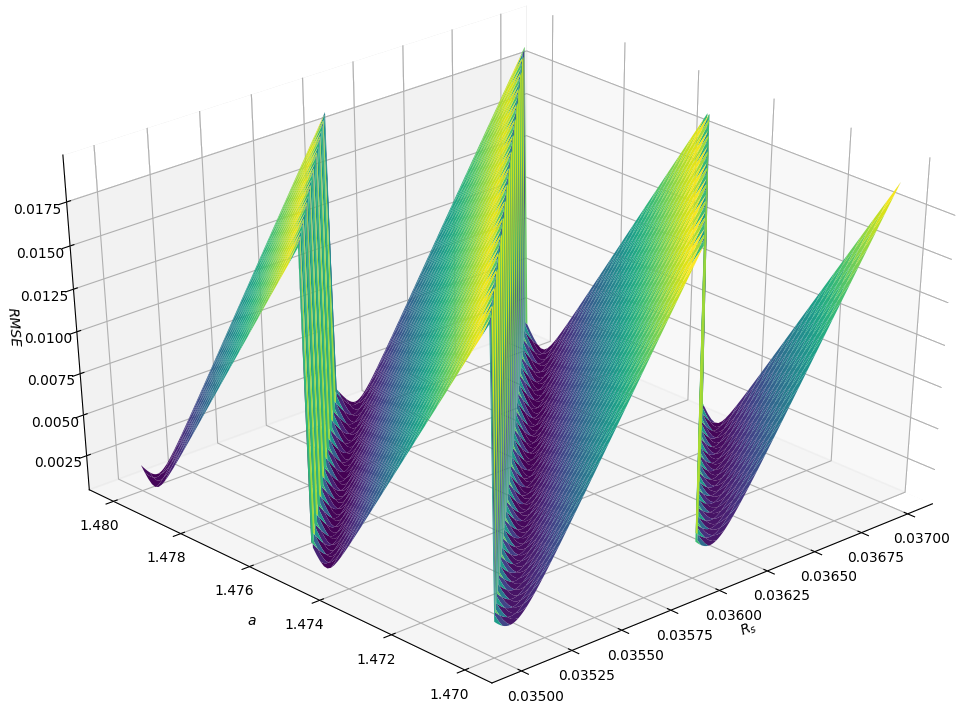
\includegraphics[width=0.5\textwidth]{resources/RTCFrance/singled/neighborhood.png}
    \caption{Le voisinage du minimum global retrouvé par l'ED selon le facteur d'idéalité et la résistance en série. Notons l'existence des "vallées" qui comprennent potentiellement plusieurs minimums locaux}
    \label{fig:neigh}
  \end{center}
\end{figure}

La nature stochastique de l'Évolution Différentielle fait qu'elle donne des résultats différents après chaque essai. Ceci impose une analyse de cohérence de la méthode pour estimer la fiabilité de l'ED pendant plusieurs essais consécutifs. Figure \ref{fig:consist} montre la RMSE de la solution finale dans 30 essais indépendants de l'ED.
Tous les points sont localisés dans une région très concentrée de l'espace de recherche ce qui indique que l'ED parvient effectivement à localiser le minimum global.
Les écart-types des paramètres montrés sur le tableau \ref{tab:RTCstats} confirment ceci puisque ils peuvent être interprétés comme un indice de "stabilité" de l'algorithme qui quantifié sa capacité a reproduire les mêmes résultats. Tous les écart-types sont de l'ordre de $10^{-3}$ ou moins, donc une solution précise est garantie dans n'importe quel essai.

\begin{figure}
    \begin{center}
      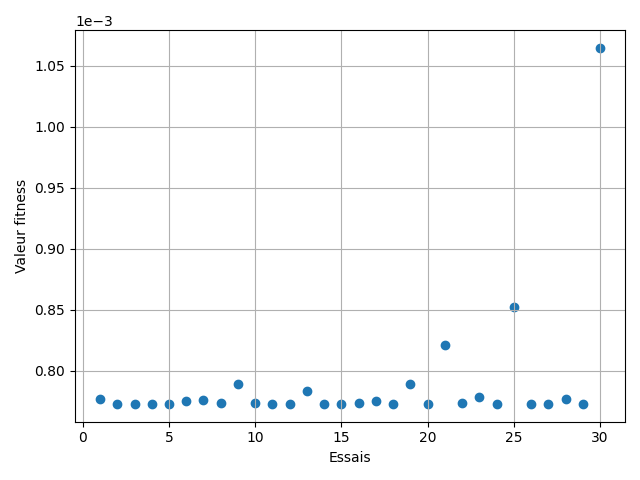
\includegraphics[width=.5\textwidth]{resources/RTCFrance/singled/consist.png}
      \caption{Les RMSEs obtenues lors de 30 essais indépendants sur la cellule RTC France 57 mm}
      \label{fig:consist}
    \end{center}
  \end{figure} 

\begin{table}
  \caption{Valeurs Moyennes de quelques paramètres influents de la cellule RTC France 57 mm et les écart-types associés des 30 essais}
  \label{tab:RTCstats}

  \begin{center}
    \begin{tabular*}{.7\textwidth}{c@{\extracolsep{\fill}}cc}
       \hline
       Paramètre & Valeur Moyenne & Écart-Type\\
       \hline
       $RMSE$       & \num{7.8925e-04}       & \num{5.3670e-05} \\
       $R_s$        & \num{3.6355e-02}       & \num{3.8936e-04} \\
       $a$          & \num{1.4722}           & \num{5.7539e-03} \\
       $I_0$        & \num{3.2655e-07}       & \num{3.4071e-08} \\
       \hline
    \end{tabular*}
  \end{center}
\end{table}

\section{Utilisation de l'outil \textit{DEPV}}

\section{Conclusion}

Le modèle double diode contient deux termes exponentiels nécessitant deux évaluations de la fonction W de Lambert pour chaque point expérimental, ce qui est relativement coûteux d'un point de vue de calcul numérique. Par ailleurs, puisque tous les parametres sont traités indépendamment des autres, l'espace de recherche est effectivement à 7 dimensions. Puisque la qualité des résultats des modèles simple et double diode est quasi-identique dans le cas de la cellule RTC France (Tableaux \ref{tab:RTCres} et \ref{tab:RTCresdouble} respectivement) ainsi que pour le module photovoltaïque monocristallin Schutten Solar STM6-40/36 (Tableaux \ref{tab:stm6} et \ref{tab:STM6double}), on constate que le modèle simple diode et très adéquat en terme de précision et supérieur en terme d'efficacité et rapidité de calcul.

  \chapter{Résultats et analyse}

\section{Introduction}
Dans ce chapitre final nous allons analyser et discuter les résultats de l'application de l'ED. Les cas d'études considérés sont une cellule très largement étudiée dans la littérature (R.T.C France 57 mm) et des module PV en mono-Si (Schutten Solar STM6-40/36) et poly-Si (Photowatt-PWP 201). On effectue aussi une analyse sur la stabilité et cohérence de la méthode avant de conclure avec une comparaison entre la méthode standard et la stratégie métaheuristique proposée à la fin du troisième chapitre. Tous les calculs ont été effectués et les résultats obtenus avec \textit{Python 3.8.3} (implementation standard \textit{CPython}) et un processeur \textit{Intel i5-7200U} avec une fréquence d'horloge maximale de 3.1\si{\giga\hertz} sous le système d'exploitation \textit{Arch Linux x86\_64} Kernel version \textit{5.7.2 arch1-1.}

\section{Cas d'études et résultats}
\subsection{Cas 1: Cellule 57-mm de R.T.C France}

Ce premier cas d'étude concerne la cellule en silicium de R.T.C France avec un diamètre de 57 mm qui a été très largement étudiée dans la littérature. Sa courbe caractéristique a été mesurée dans des conditions de température $T = \SI{33}{\celsius}$ et irradiance solaire $\SI{1000}{\watt\per\square\meter}$ et comprend 26 points expérimentaux dont 20 est dans le premier quadrant (figure \ref{fig:RTCexp}). Le tableau \ref{tab:singleboundaries} montre le bornes de l'espace de recherche et figure \ref{fig:RTCres} prouve que la caractéristique expérimentale et calculée par l'ED sont graphiquement quasi-identiques. Figure \ref{fig:RTCres}.b montre l'évolution de la moyenne des valeurs de fitness des vecteurs évalués par la fonction objectif dans chaque génération consécutive. On constate que dès la 50\textsuperscript{ème} génération, l'ED a pratiquement déjà convergé.

Le tableau \ref{tab:RTCres} présente une comparaison entre l'ED et d'autre méthodes simple diode appliquées à la cellule R.T.C France. On constate que les valeurs retrouvées par l'ED sont assez proches de celles des autres travaux. En effet, l'ED parvient à une erreur RMSE de \num{7.7692e-04} qui est supérieure aux autres techniques similaire comme les essaims particulaires \cite{Hamid2016}, l'algorithme des colonies d'abeilles artificielles \cite{Oliva2014} et l'ED à trois points \cite{Chin2019}. Les résultats les moins précis sont ceux de la méthode de Newton à moindres carrés \cite{Easwarakhanthan1986} et l'algorithme génétique \cite{Oliva2014}.

\begin{table}
  \caption{Bornes utilisées de l'espace de recherche pour le modèle simple diode pour le cellule R.T.C France}
  \label{tab:singleboundaries}

  \begin{center}
    \begin{tabular*}{\textwidth}{l@{\extracolsep{\fill}}lllll}
       \hline
       Paramètre         & $R_s$ & $R_{p}$ & $a$ & $I_0$      & $I_{PV}$ \\
       \hline
       Borne supérieure  & 1     & 100      & 2   & \num{1e-06}& 10\\
       Borne inférieure  & 0     & 2        & 1   & \num{1e-07}& 0 \\
       \hline
    \end{tabular*}
  \end{center}
\end{table}

\begin{figure}
  \begin{center}
    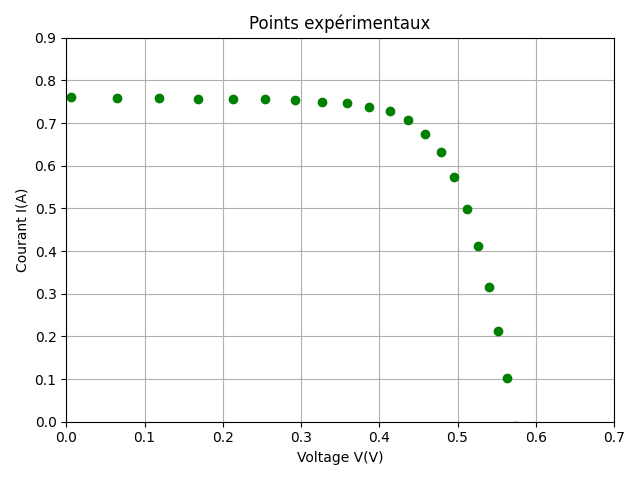
\includegraphics[width=0.5\textwidth]{resources/RTCFrance/exp.png}
    \caption{Données expérimentales de la caractéristique IV de la cellule R.T.C France mesurées à \SI{33}{\celsius}}
    \label{fig:RTCexp}
  \end{center}
\end{figure}

\begin{figure*}
    \centering
    \begin{subfigure}[b]{0.45\textwidth}
        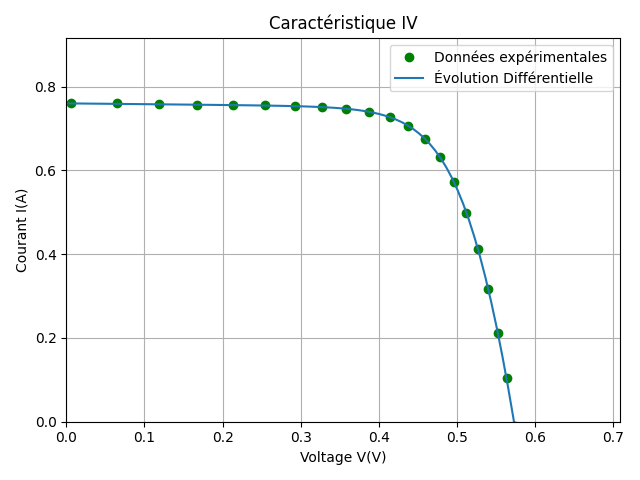
\includegraphics[width=\textwidth]{resources/RTCFrance/singled/iv.png}
        \caption{Comparaison entre la courbe expérimentale et la caractéristique calculée.}
    \end{subfigure}
    ~
    \begin{subfigure}[b]{0.45\textwidth}
        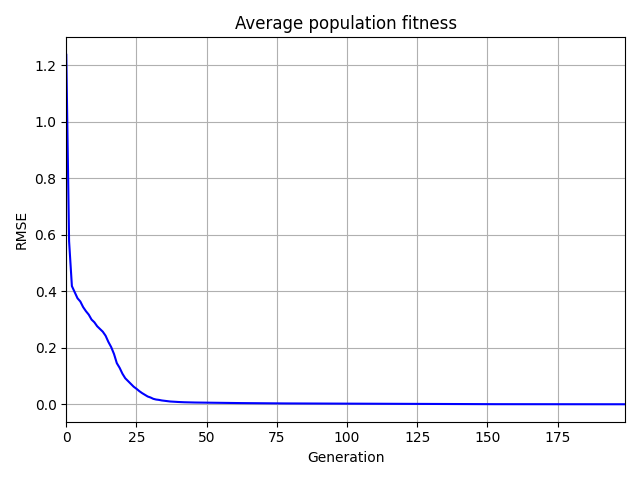
\includegraphics[width=\textwidth]{resources/RTCFrance/singled/fitness.png}
        \caption{Évolution de la valeur moyenne de fitness de chaque génération}
    \end{subfigure}
    \caption{Résultats de l'ED appliquée sur la cellule R.T.C France 57 mm.}
    \label{fig:RTCres}
\end{figure*}

\begin{table}
  \caption{Comparaison de l'ED avec d'autres méthodes utilisant le modèle simple diode appliquées à la cellule R.T.C France 57 mm dans la littérature}
  \label{tab:RTCres}

  \begin{center}
  \scriptsize
    \begin{tabular*}{\textwidth}{l@{\extracolsep{\fill}}cllllll }
       \hline
       Paramètres & Référence & $R_s$ (\si{\ohm}) & $R_{p} (\si{\ohm})$ & $a $ & $I_0$ (\si{\micro\ampere}) & $I_{PV}$ (\si{\ampere}) & $RMSE$ \\
       \hline
       ED (simple diode) &                            & \num{0.0363} & \num{54.1134} & \num{1.4709} & \num{0.3209} & \num{0.7607} & \num{7.7692e-04}\\
       ED3P              & \cite{Chin2019}            & \num{0.0363} & \num{54.1924} & \num{1.4798} & \num{0.3191} & \num{0.7607} & \num{8.1291e-04}\\
       PSO               & \cite{Hamid2016}           & \num{0.0363} & \num{53.8550} & \num{1.4816} & \num{0.3245} & \num{0.7607} & \num{9.8606e-04}\\
       ABC               & \cite{Oliva2014}           & \num{0.0364} & \num{53.6433} & \num{1.4817} & \num{0.3251} & \num{0.7608} & \num{9.8620e-04}\\
       Newton            & \cite{Easwarakhanthan1986} & \num{0.0364} & \num{53.7634} & \num{1.4837} & \num{0.3223} & \num{0.7608} & \num{9.70e-03}  \\
       GA                & \cite{Oliva2014}           & \num{0.0299} & \num{42.3729} & \num{1.5751} & \num{0.8087} & \num{0.7619} & \num{1.90e-02}  \\
       \hline
    \end{tabular*}
  \end{center}
\end{table}

\nomenclature{ED3P}{Évolution différentielle à trois points}
\nomenclature{ABC}{Colonies d'abeilles artificielles (\textit{Artificial Bee Colony Optimization})}

En ce qui concerne le modèle double diode, les paramètres sont contraints dans les limites dans le tableau \ref{tab:doubledboundaries}. Les résultats de l'ED en double diode sont comparés avec ceux de quelques autres méthode dans le tableau \ref{tab:RTCresdouble}.
\begin{table}
  \caption{Bornes de l'espace de recherche à 7 dimensions pour la cellule R.T.C France 57mm}
  \label{tab:doubledboundaries}

  \begin{center}
  \small
    \begin{tabular*}{\textwidth}{l@{\extracolsep{\fill}}lllllll}
      \hline
      Paramètre & $R_s$ & $R_{p}$ & $a_1$ & $a_2$ & $I_{01}$   & $I_{02}$    & $I_{PV}$ \\
      \hline
      Borne supérieure  & 1     & 100      & 2     & 2     & \num{1e-04}& \num{1e-04} & 10 \\
      Borne inférieure  & 0     & 2        & 1     & 1     & \num{1e-07}& \num{1e-07} & 0  \\
      \hline
    \end{tabular*}
  \end{center}
\end{table}

\begin{table}
  \caption{Comparaison de l'ED avec d'autres méthodes dans la littérature utilisant le modèle double diode sur la cellule R.T.C France 57mm}
  \label{tab:RTCresdouble}

  \begin{center}
  \scriptsize
    \begin{tabular*}{\textwidth}{l@{\extracolsep{\fill}}cllllllll}
       \hline
       Paramètres & Référence & $R_s$ (\si{\ohm}) & $R_{p} (\si{\ohm})$ & $a_1$ & $a_2$ & $I_{01}$ (\si{\ampere}) & $I_{02}$ (\si{\ampere}) & $I_{PV}$ (\si{\ampere}) & $RMSE$ \\
       \hline
       ED (double diode) &                            & \num{0.02061}   & \num{51.9345} & \num{1.87579} & \num{1.43602} & \num{4.2322e-07} 
                                                      & \num{1.8726e-07}& \num{0.76055} & \num{7.63e-04}   \\
       ABC               & \cite{Oliva2014}           & \num{0.0364}    & \num{53.7804} & \num{1.4495} & \num{1.4885} & \num{4.07e-08}
                                                      & \num{2.874e-07} & \num{0.7608}  & \num{9.861e-04}\\
       PSO               & \cite{Jordehi2016}         & \num{0.05861}   & \num{18.2106} & \num{1.00012} & \num{1.00091} & \num{2.8601e-10} 
                                                      & \num{1e-12}     & \num{0.7633}  & \num{8.1646e-03} \\
       GSA               & \cite{Jordehi2017}         & \num{0.02914}   & \num{51.116}  & \num{1.6087}  & \num{1.62889} & \num{6.60621e-7} 
                                                      & \num{4.55149e-7}& \num{0.76886} & \num{5.91958e-03}\\
       \hline
    \end{tabular*}
  \end{center}
\end{table}

\nomenclature{GSA}{Gravitational Search Algorithm}

\subsection{Cas 2: Module monocristallin Schutten Solar STM6-40/36}

Nous nous concernons dans ce deuxième cas d'étude du module monocristallin Schutten Solar STM6-40/36 composé de 36 cellules ($156\si{\milli\meter}\times 156\si{\milli\meter}$) en série. Les données expérimentales ont été prises à une température de 51\si{\celsius}. Une comparaison des résultats de l'ED avec d'autres méthodes est présentée dans le tableau \ref{tab:stm6}. La correspondance de la caractéristique calculée par l'ED aux points experimentaux est démontrée graphiquement dans la figure \ref{fig:STM6res}. Malgré la distribution irrégulière des points, l'ED arrive a produire une solution précise. Sa précision et de même ordre de grandeur que ED3P \cite{Chin2019} mais elle est supérieure aux techniques des colonies des abeilles artificielles (ABC) \cite{Oliva2014}, de sa version améliorée par Oliva et al. (CIABC) \cite{Oliva2017a} et Chaotic Whale Optimization Algorithm (CWOA) \cite{Oliva2017}.
\begin{figure*}
    \centering
    \begin{subfigure}[b]{0.45\textwidth}
        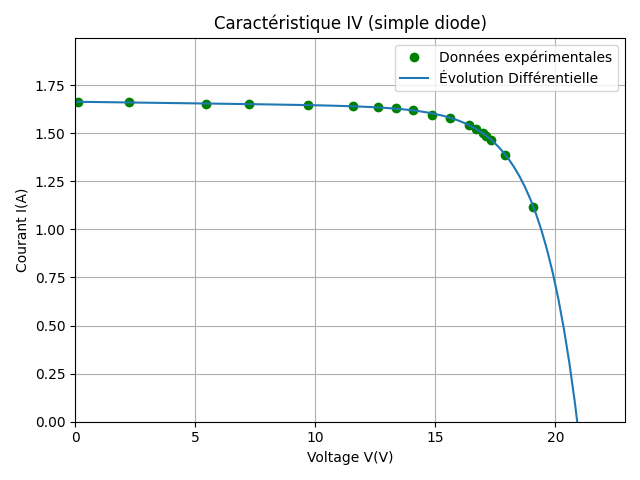
\includegraphics[width=\textwidth]{resources/STM6/singled/iv.png}
        \caption{Correspondence de l'ED aux données expérimentales. La distribution non-optimale des points n'entrave pas la convergence.}
    \end{subfigure}
    ~
    \begin{subfigure}[b]{0.45\textwidth}
        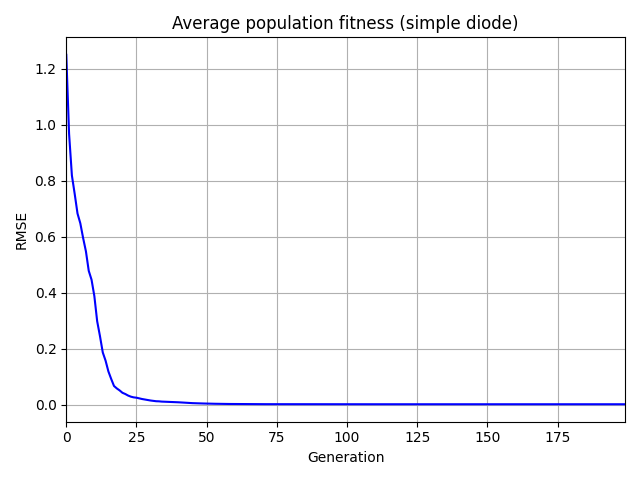
\includegraphics[width=\textwidth]{resources/STM6/singled/fitness.png}
        \caption{Évolution de la valeur moyenne de fitness de chaque génération. L'ED est convergeante dès la $50^{\text{ème}}$ itération.}
    \end{subfigure}
    \caption{Résultats de l'ED appliquée sur au module Schutten Solar STM6-40/36}
    \label{fig:STM6res}
\end{figure*}
\begin{table}
  \caption{Comparaison de l'ED (simple diode) avec d'autres méthodes dans la littérature sur le module STM6-40/36}
  \label{tab:stm6}

  \begin{center}
    \scriptsize
    \begin{tabular*}{\textwidth}{l@{\extracolsep{\fill}}cllllll}
      \hline
      Paramètres & Référence & $R_s$ (\si{\milli\ohm}) & $R_{p} (\si{\ohm})$ & $a $ & $I_0$ (\si{\micro\ampere}) & $I_{PV}$ (\si{\ampere}) & $RMSE$ \\
      \hline
       ED (simple diode)  &                   & \num{0.2801} & \num{16.5854} & \num{1.5571} & \num{2.8049} & \num{1.6633} & \num{1.7721e-03}  \\
       ED3P               & \cite{Chin2019}   & \num{0.4186} & \num{16.7328} & \num{1.5656} & \num{2.7698} & \num{1.6632} & \num{1.7740e-03}  \\
       ABC                & \cite{Oliva2014}  & \num{4.99}   & \num{15.206}  & \num{1.4866} & \num{1.5}    & \num{1.6644} & \num{1.838e-03}   \\
       CIABC              & \cite{Oliva2017a} & \num{4.4}    & \num{15.617}  & \num{1.4976} & \num{1.6642} & \num{1.6760} & \num{1.819e-03}   \\
       CWOA               & \cite{Oliva2017}  & \num{5}      & \num{15.4}    & \num{1.5}    & \num{1.6338} & \num{1.7}    & \num{1.800e-03}   \\
       \hline
    \end{tabular*}
  \end{center}
\end{table}
\nomenclature{CIABC}{Chaotic Improved Artificial Bee Colony}
\nomenclature{CWOA}{Chaotic Whale Optimization Algorithm}


Les résultats de l'ED avec le modèle double diode sur le module STM6-40/36 sont présenté dans le tableau \ref{tab:STM6double} avec deux autres techniques: La colonie d'abeilles artificielle et les essaims particulaires. Le tableau \ref{tab:stm6doublelimits} montre les bornes utilisées comme limites de l'espace de recherche. Notons la similarité des qualités des résultats du modèle simple et double diode.
\begin{table}
  \caption{Limites de l'espace de recherche pour l'ED double diode sur le module photovoltaïque STM6-40/36}
  \label{tab:stm6doublelimits}

  \begin{center}
    \begin{tabular*}{\textwidth}{l@{\extracolsep{\fill}}lllllll}
      \hline
      Paramètre         & $R_s$ & $R_{p}$ & $a_1$ & $a_2$ & $I_{01}$   & $I_{02}$    & $I_{PV}$ \\
      \hline
      Borne Supérieure  & 1     & 100      & 2     & 2     & \num{1e-04}& \num{1e-04} & 10\\
      Borne inférieure  & 0     & 2        & 1     & 1     & 0          & 0           & 0\\
      \hline
    \end{tabular*}
  \end{center}
\end{table}
\begin{table}
  \caption{Comparaison de l'ED (double diode) avec d'autres méthodes sur le module photovoltaïque STM6-40/36}
  \label{tab:STM6double}

  \begin{center}
  \scriptsize
    \begin{tabular*}{\textwidth}{l@{\extracolsep{\fill}}cllllllll}
       \hline
       Paramètres & Référence & $R_s$ (\si{\ohm}) & $R_{p} (\si{\ohm})$ & $a_1$ & $a_2$ & $I_{01}$ (\si{\ampere}) & $I_{02}$ (\si{\ampere}) & $I_{PV}$ (\si{\ampere}) & $RMSE$ \\
       \hline
       ED (double diode) &                            & \num{0.0177}    & \num{16.7050}& \num{1.9049} & \num{1.52461}   & \num{1.006e-06} 
                                                      & \num{2.9858e-06}& \num{1.6633} & \num{1.7724e-03}   \\
       ELPSO             & \cite{RezaeeJordehi2018}   & \num{0.0138}    & \num{16.8580}& \num{1.8706} & \num{1.16648}   & \num{1.670e-08} 
                                                      & \num{6.21092e-6}& \num{1.6648} & \num{1.8307e-03}   \\
       ABC               & \cite{RezaeeJordehi2018}   & \num{0.03434}   & \num{26.0613}& \num{1.9851}  & \num{1.4687}** & \num{8.938e-6} 
                                                      & \num{1e-12}     & \num{1.66347}& \num{2.0538e-03}\\
       \hline
    \end{tabular*}
  \end{center}
\end{table}
\nomenclature{ELPSO}{Enhanced Leader Particle Swarm Optimization}

\subsection{Cas 3: Module polycristallin Photowatt-PWP 201}

\begin{figure*}
    \centering
    \begin{subfigure}[b]{0.45\textwidth}
        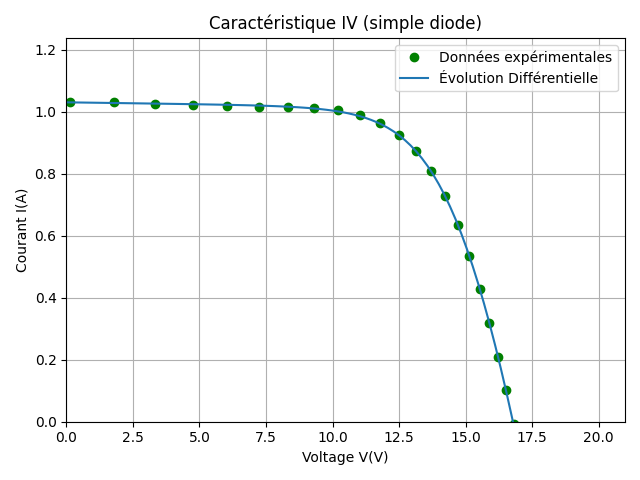
\includegraphics[width=\textwidth]{resources/pwp/iv.png}
        \caption{Caractéristique expérimentale et calculée du module polycristallin Photowatt-PWP 201.}
    \end{subfigure}
    ~
    \begin{subfigure}[b]{0.45\textwidth}
        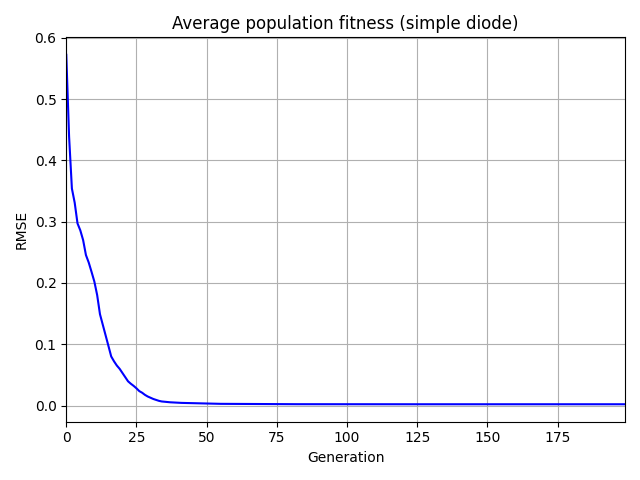
\includegraphics[width=\textwidth]{resources/pwp/fitness.png}
        \caption{Courbe de convergence de L'ED. Notons la convergence rapide (avant $< 100$ itérations)}
    \end{subfigure}
    \caption{Résultats de l'ED appliquée sur au module Photowatt PWP-201}
    \label{fig:pwpsingle}
\end{figure*}
Le 3\textsuperscript{ème} cas concerne le module polycristallin Photowatt-PWP 201 composé de 36 cellules en série. Les données expérimentales ont été prise dans des conditions d'irradiation de $1000 \si{\watt\per\square\meter}$ et une température de $T = 45 \si{\celsius}$. Le tableau \ref{tab:pwpsingle} compare les résultats obtenus par Évolution Différentielle contre d'autres méthodes dans la littérature. Les valeurs des paramètres simple diode retrouvée par l'ED sont très similaires aux autres, mais sont plus précises en termes de RMSE. Figure \ref{fig:pwpsingle} montre la courbe caractéristique calculée (a) et la courbe de convergence de l'ED (b). Les bornes de l'espace de recherche sont identiques à celle de la cellule R.T.C France (Tableau \ref{tab:singleboundaries}) sauf pour le courant de saturation qu'on limite à $\num{1e-7} \leq I_{0} \leq \num{1e-5}$. Le modèle double diode est plus précis que le modèle simple diode avec l'ED, mais ce dernier reste plus précis avec l'ED que les autres techniques utilisant le modèle simple diode.

\begin{table}
  \caption{Comparaison de l'ED avec d'autres méthodes simple diode dans la littérature sur le module Photowatt-PWP 201}
  \label{tab:pwpsingle}

  \begin{center}
    \scriptsize
    \begin{tabular*}{\textwidth}{l@{\extracolsep{\fill}}cllllll}
      \hline
      Paramètres & Référence & $R_s$ (\si{\milli\ohm}) & $R_{p} (\si{\ohm})$ & $a $ & $I_0$ (\si{\micro\ampere}) & $I_{PV}$ (\si{\ampere}) & $RMSE$ \\
      \hline
       ED (simple diode)  &                   & \num{0.0343} & \num{22.8238} & \num{1.3139} & \num{2.6380} & \num{1.0314} & \num{2.0529e-03}  \\
       ED3P               & \cite{Chin2019}   & \num{0.0347} & \num{19.3720} & \num{1.3002} & \num{2.1247} & \num{1.0335} & \num{2.4227e-03}  \\
       ISCE               & \cite{Gao2018}    & \num{0.0333} & \num{27.2772} & \num{1.3512} & \num{3.4823} & \num{1.0305} & \num{2.4251e-03}  \\
       CIABC              & \cite{Wu2018}     & \num{0.0333} & \num{27.2772} & \num{1.3512} & \num{3.4822} & \num{1.0305} & \num{2.425e-03}   \\
       Newton     & \cite{Easwarakhanthan1986}& \num{0.0335} & \num{15.2625} & \num{1.3458} & \num{3.2876} & \num{1.0318} & \num{5.6010e-01}  \\
       \hline
    \end{tabular*}
  \end{center}
\end{table}
\begin{table}
  \caption{Comparaison de l'ED avec d'autres méthodes double diode sur le module photovoltaïque Photowatt-PWP 201}
  \label{tab:pwpdouble}

  \begin{center}
  \scriptsize
    \begin{tabular*}{\textwidth}{l@{\extracolsep{\fill}}cllllllll}
       \hline
       Paramètres & Référence & $R_s$ (\si{\ohm}) & $R_{p} (\si{\ohm})$ & $a_1$ & $a_2$ & $I_{01}$ (\si{\ampere}) & $I_{02}$ (\si{\ampere}) & $I_{PV}$ (\si{\ampere}) & $RMSE$ \\
       \hline
       ED (double diode) &                            & \num{0.8604}    & \num{19.2098}& \num{1.2165} & \num{1.5326}    & \num{1.6785e-7} 
                                                      & \num{2.6073e-06}& \num{1.03193}& \num{1.50208e-03}   \\
       TVACPSO           & \cite{Jordehi2016}         & \num{1.2356}    & \num{22.8236}& \num{1.3210} & \num{2.7778}   & \num{2.6381e-6} 
                                                      & \num{1e-12}     & \num{1.03143}& \num{2.0530e-03}   \\
       %ABC               & \cite{RezaeeJordehi2018}   & \num{0.03434}   & \num{26.0613}& \num{1.9851}  & \num{1.4687}** & \num{8.938e-6} 
       %                                               & \num{1e-12}     & \num{1.66347}& \num{2.0538e-03}\\
       \hline
    \end{tabular*}
  \end{center}
\end{table}

\subsection{Remarques}
Le modèle double diode contient deux termes exponentiels nécessitant deux évaluations de la fonction W de Lambert pour chaque point expérimental, ce qui est relativement coûteux d'un point de vue de calcul numérique. Par ailleurs, puisque tous les paramètres sont traités indépendamment des autres, l'espace de recherche est effectivement à 7 dimensions. Puisque la qualité des résultats des modèles simple et double diode est quasi-identique dans le cas de la cellule R.T.C France (Tableaux \ref{tab:RTCres} et \ref{tab:RTCresdouble} respectivement) ainsi que pour le module photovoltaïque monocristallin Schutten Solar STM6-40/36 (Tableaux \ref{tab:stm6} et \ref{tab:STM6double}), on constate que le modèle simple diode et très adéquat en terme de précision et supérieur en terme d'efficacité et rapidité de calcul.

\section{Analyse et cohérence de l'ED}

La performance supérieure démontrée par l'ED par rapport aux autres algorithmes provient probablement de ses capacités à la \textit{recherche globale} et l'auto-adaptation permise par les vecteurs de différences qui permettent au début d'explorer tout l'espace de recherche, et se raffinent progressivement pour optimiser la recherche locale dans la région du minimum global. L'existence d'une multitude de minimums locaux est démontrée dans la figure \ref{fig:neigh} où on a projeté l'espace de recherche 5-dimensionnel sur 2 dimensions au voisinage du minimum global. On fait varier le facteur d'idéalité $a$ et la résistance série $R_s$ dont le modèle est très sensible aux variations. Les trois autres paramètres $R_{p}$, $I_0$ et $I_{PV}$ sont fixés sur les valeurs du minimum global retrouvé par l'ED comme dans le tableau \ref{tab:RTCres}.

\begin{figure}
  \begin{center}
    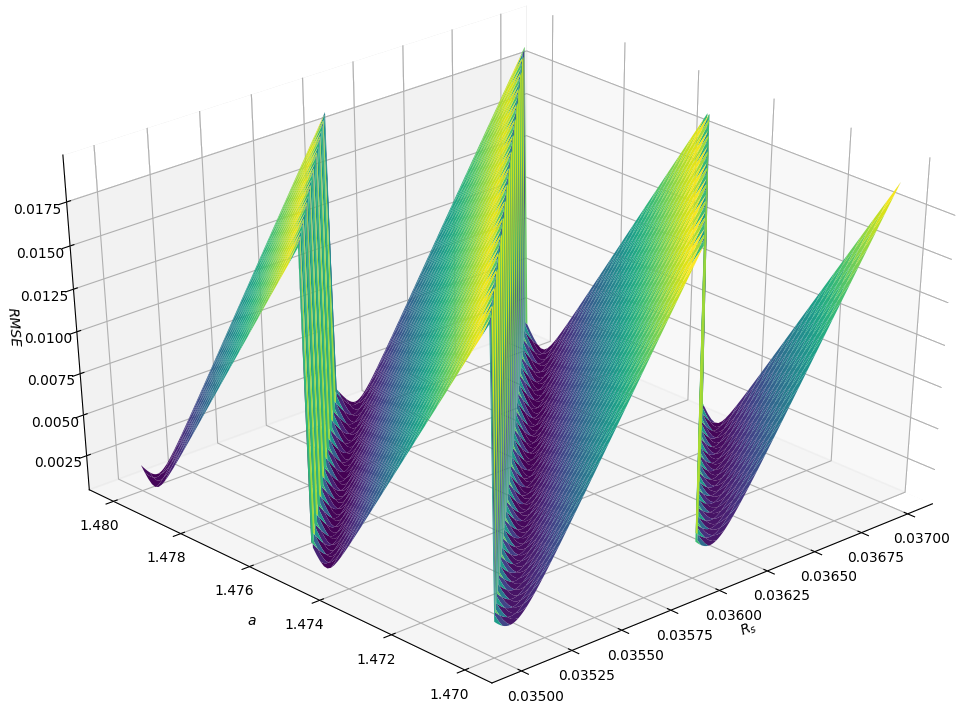
\includegraphics[width=0.7\textwidth]{resources/RTCFrance/singled/neighborhood.png}
    \caption{Le voisinage du minimum global retrouvé par l'ED selon le facteur d'idéalité et la résistance en série. Notons l'existence des "vallées" qui comprennent potentiellement plusieurs minimums locaux}
    \label{fig:neigh}
  \end{center}
\end{figure}

La nature stochastique de l'Évolution Différentielle fait qu'elle donne des résultats différents après chaque essai. Ceci impose une analyse de cohérence de la méthode pour estimer la fiabilité de l'ED pendant plusieurs essais consécutifs. Figure \ref{fig:consist} montre la RMSE de la solution finale dans 30 essais indépendants de l'ED.
Tous les points sont localisés dans une région très concentrée de l'espace de recherche ce qui indique que l'ED parvient effectivement à localiser le minimum global.
La cohérence des différents essais concernant la $R_s$ et le $a$ du module Photowatt-PWP 201 (Figure \ref{fig:paramconsist}) et les écart-types des paramètres montrés sur le tableau \ref{tab:RTCstats} confirment ceci puisque ils peuvent être interprétés comme un indice de "stabilité" de l'algorithme qui quantifie sa capacité a reproduire les mêmes résultats. Tous les écart-types sont de l'ordre de $10^{-3}$ ou moins, donc une solution précise est garantie dans n'importe quel essai.

\begin{figure*}
    \centering
    \begin{subfigure}[b]{0.45\textwidth}
        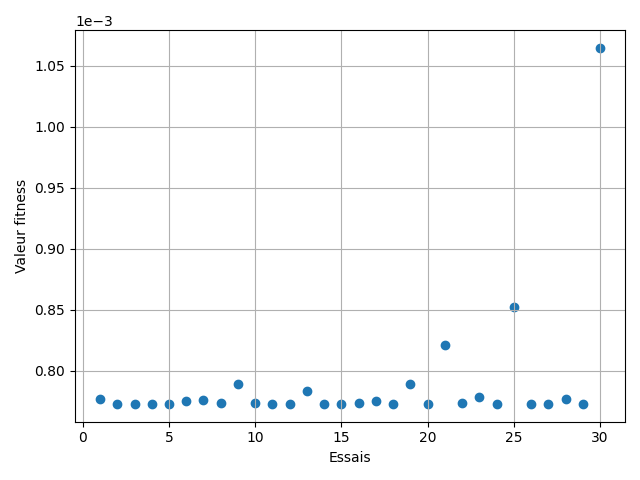
\includegraphics[width=\textwidth]{resources/RTCFrance/singled/consist.png}
        \caption{Cellule R.T.C France 57 mm}
    \end{subfigure}
    ~
    \begin{subfigure}[b]{0.45\textwidth}
        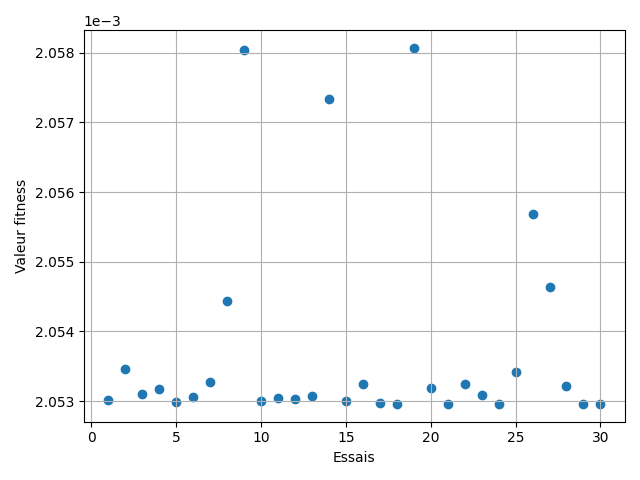
\includegraphics[width=\textwidth]{resources/pwp/consistency.png}
        \caption{Module Photowatt-PWP 201}
    \end{subfigure}
    \caption{Les RMSEs obtenues lors de 30 essais indépendants}
    \label{fig:consist}
\end{figure*}

\begin{figure*}
    \centering
    \begin{subfigure}[b]{0.45\textwidth}
        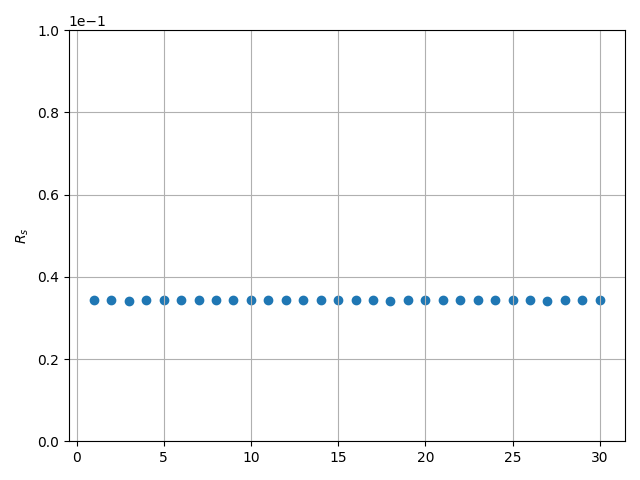
\includegraphics[width=\textwidth]{resources/pwp/rsconsist.png}
        \caption{Résistance série $R_s$}
    \end{subfigure}
    ~
    \begin{subfigure}[b]{0.45\textwidth}
        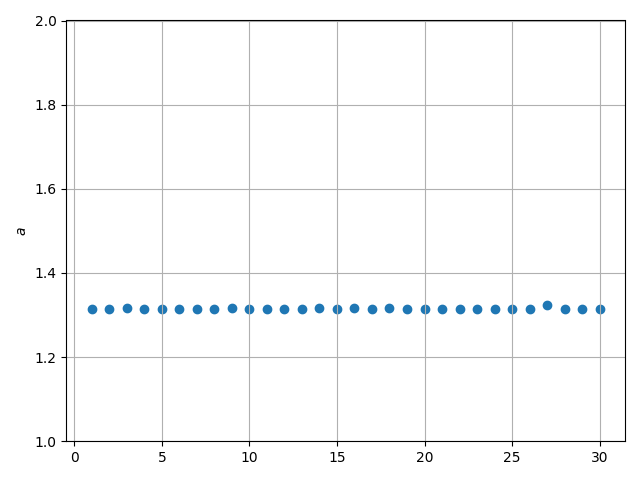
\includegraphics[width=\textwidth]{resources/pwp/aconsist.png}
        \caption{Facteur d'idéalité $a$}
    \end{subfigure}
    \caption{Résultats obtenus pour le facteur d'idéalité et la résistance série du module Potowatt-PWP 201 pendant 30 essais indépendants}
    \label{fig:paramconsist}
\end{figure*}

\begin{table}
  \caption{Valeurs Moyennes de quelques paramètres influents de la cellule R.T.C France 57 mm et les écart-types associés des 30 essais}
  \label{tab:RTCstats}
  \small
  \begin{center}
    \begin{tabular*}{.7\textwidth}{c@{\extracolsep{\fill}}cc}
       \hline
       Paramètre & Valeur Moyenne & Écart-Type\\
       \hline
       $RMSE$       & \num{7.8925e-04}       & \num{5.3670e-05} \\
       $R_s$        & \num{3.6355e-02}       & \num{3.8936e-04} \\
       $a$          & \num{1.4722}           & \num{5.7539e-03} \\
       $I_0$        & \num{3.2655e-07}       & \num{3.4071e-08} \\
       \hline
    \end{tabular*}
  \end{center}
\end{table}

\section{Analyse de la stratégie métaheuristique}
Pour analyser la stratégie métaheuristique proposée dans le dernier chapitre, nous allons prendre le module polycristallin Photowatt-PWP 201 et la cellule R.T.C France 57mm.
Conformément aux recommandations de Storn et Price, nous avons choisi comme valeurs standard du facteur de mutation et du taux de croisement $0.7$ et $0.8$, respectivement. En fait les paramètres retrouvés dans le cas d'étude 3 avec les courbes caractéristique et de convergence, ont tous été retrouvé par l'ED configuré avec ces valeurs par défaut. Pour appliquer la métaheuristique, un nombre de population relativement faible est adéquat puisque notre espace de recherche est 2-dimensionnel: $N_P^{\text{higher order}} = 10 \times D = 20$. On limite aussi le nombre maximal de générations à $Gen_{max}^{\text{higher order}} = 50$. Pratiquement, la fonction objectif est donc la valeur fitness \textit{à la 50\textsuperscript{ème} itération}. Le fait que l'ED risque de ne pas avoir déjà convergé ne nous pose pas de problèmes, puisque notre but est de retrouver les valeurs de $F$ et $CR$ permettant la convergence la plus rapide\footnote{Convergence rapide mais non-prematurée} que possible. Les paramètres de la métaheuristique elle-même sont $F^{\text{higher order}} = 0.8$ et $CR^{\text{higher order}} = 0.8$. 
Les résultats de cette stratégies sont:

\begin{eqnarray}
  F &=& 0.55, \quad CR = 0.94 \quad \text{Module Photowatt-PWP 201}\\
  F &=& 0.55, \quad CR = 0.88 \quad \text{Cellule R.T.C France 57mm}
\end{eqnarray}

Les figures \ref{fig:metaconv} et \ref{fig:metaconv2} comparent les courbes de convergences entre l'ED avec et sans stratégie métaheuristique. Malgré le fait que le facteur de mutation retrouvé est relativement relativement inférieur aux recommandations de Storn et Price, il est toujours compris dans les limites de Zaharie et al. \cite{Zaharie2002}. Notons que la rapidité de convergence est sensiblement supérieure dans les figures \ref{fig:metaconv} et \ref{fig:metaconv2}, l'ED a déjà convergé à l'itération 25, alors que l'ED standard a besoin de plus de deux fois plus d'itérations\footnote{Itérations et générations sont équivalentes dans ce cas}. En terme de temps de calcul, on teste dans les mêmes conditions les deux méthodes en les "chronométrant" avec script Python. L'ED standard s'exécute au bout d'un temps moyen de $1.68535 \si{\second}$ sur 30 essais indépendants et un écart-type de $\num{4.751e-4}$. Pour l'ED avec métaheuristique, le temps moyen d'exécution est $0.82392 \si{\second}$, ce qui correspond à une diminution de 51\% du temps de calcul. Il n'y a pas de compromis envers la stabilité et la cohérence puisque l'écart-type des RMSEs est $\num{4.0162e-4}$. 
% Figure \ref{fig:exectimes} montre les différents temps d'exécution pendant 30 essais avec les deux méthodes. Les valeurs initialement décroissantes sont probablement dues à l'utilisation des cache L1 et L2 du processeur.

\section{Conclusion}
Après avoir étudié la performance de l'ED sur la cellule et les deux modules photovoltaïques, on peut donc conclure que l'ED avec la fonction W de Lambert est plus précise que les autres techniques disponibles dans la littérature. La mutations différentielle apparaît très adaptée aux genres d'espaces de recherche présentés par les courbes caractéristique des cellules solaires. On a aussi utilisé une évolution différentielle à un ordre supérieur pour déterminer les paramètres optimaux des ED pour les modèles à diodes, ce qui a amélioré la convergence and réduit le temps de calcul.

\begin{figure*}
    \centering
    \begin{subfigure}[b]{0.45\textwidth}
        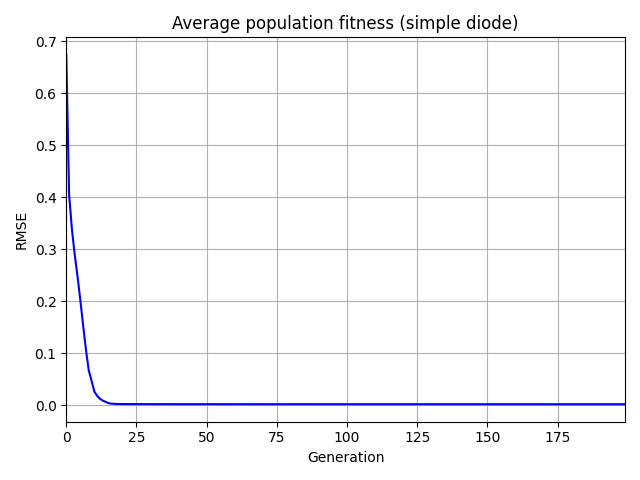
\includegraphics[width=\textwidth]{resources/pwp/metafit.png}
        \caption{Convergence de l'ED configurée avec les parametres retrouvée par la métaheuristique}
    \end{subfigure}
    ~
    \begin{subfigure}[b]{0.45\textwidth}
        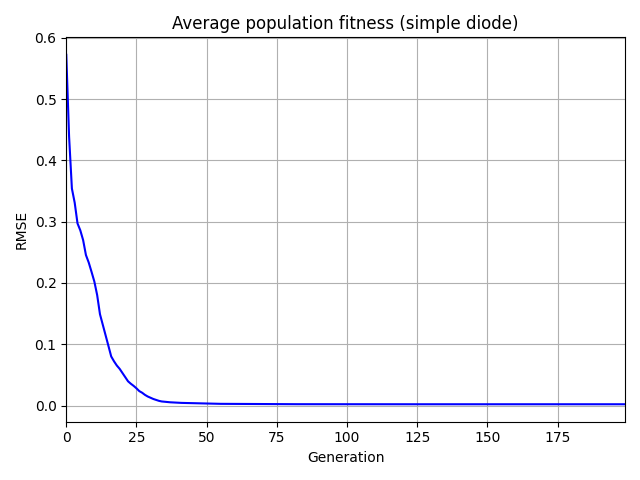
\includegraphics[width=\textwidth]{resources/pwp/fitness.png}
        \caption{Convergence de l'ED avec les paramètres standard}
    \end{subfigure}
    \caption{Comparaison de l'ED avec et sans métaheuristique sur le module Photowatt-PWP 201}
    \label{fig:metaconv}
\end{figure*}%
\begin{figure*}
    \centering
    \begin{subfigure}[b]{0.45\textwidth}
        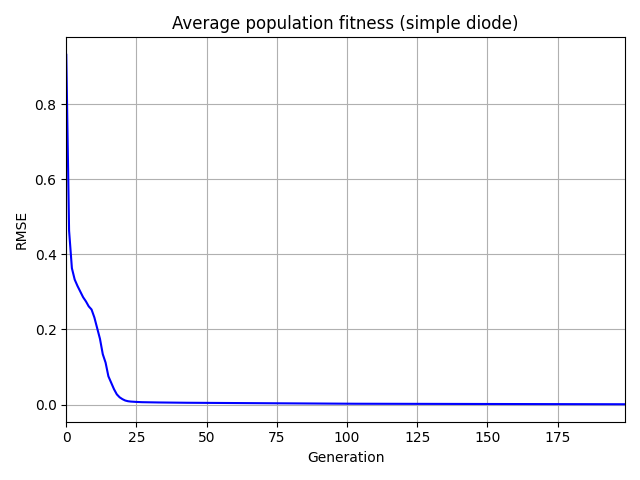
\includegraphics[width=\textwidth]{resources/RTCFrance/metaconv.png}
        \caption{Convergence de l'ED configurée avec les parametres retrouvée par la métaheuristique}
    \end{subfigure}
    ~
    \begin{subfigure}[b]{0.45\textwidth}
        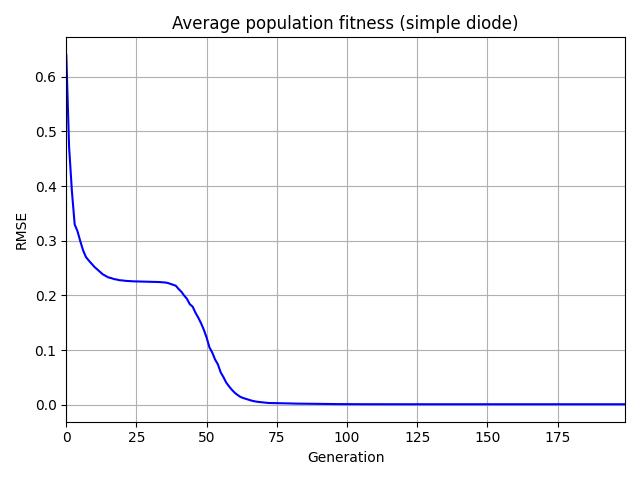
\includegraphics[width=\textwidth]{resources/RTCFrance/stdconv.png}
        \caption{Convergence de l'ED avec les paramètres standard}
    \end{subfigure}
    \caption{Comparaison de l'ED avec et sans métaheuristique sur la cellule R.T.C France 57 mm}
    \label{fig:metaconv2}
\end{figure*}%
% \begin{figure*}
%     \centering
%     \begin{subfigure}[b]{0.45\textwidth}
%         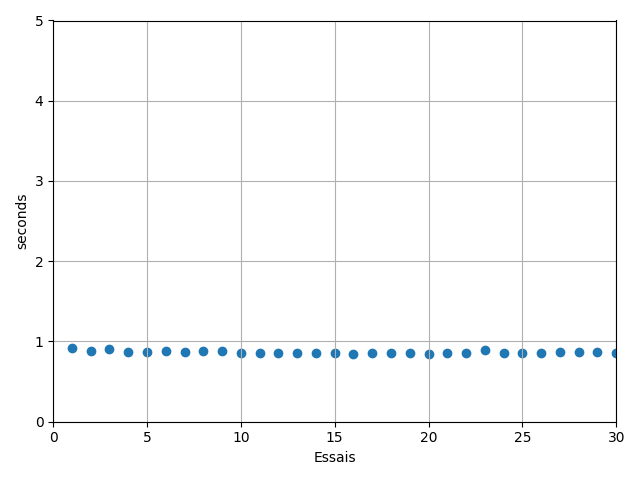
\includegraphics[width=\textwidth]{resources/metaexec.png}
%         \caption{Avec stratégie métaheuristique}
%     \end{subfigure}
%     ~
%     \begin{subfigure}[b]{0.45\textwidth}
%         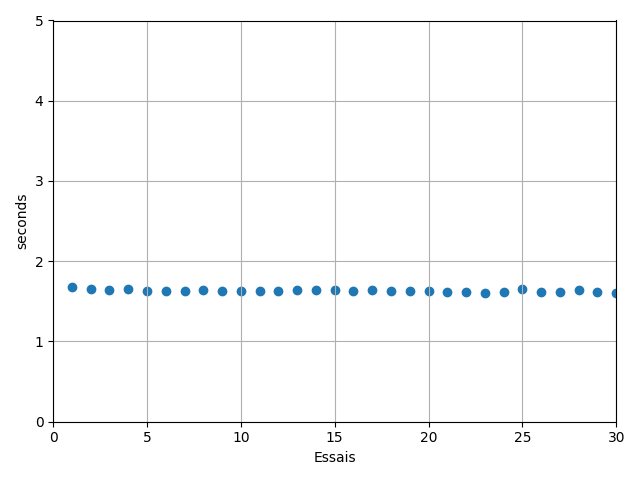
\includegraphics[width=\textwidth]{resources/stdexec.png}
%         \caption{Avec ED standard}
%     \end{subfigure}
%     \caption{Comparaison des temps de calcul pendant 30 essais}
%     \label{fig:exectimes}
% \end{figure*}

  \bibliographystyle{ieeetr}
  \bibliography{masterlibrary}
\end{document}
